%\documentclass[a4paper,10pt]{article}
\documentclass[acmcsur]{acmtrans2m}
\usepackage[utf-8]{inputenc}

\usepackage{paralist}

\usepackage{graphicx}

\usepackage{colortbl}
\usepackage{color,soul}
\usepackage{longtable}
\usepackage{pdflscape}
\newtheorem{theorem}{Theorem}[section]
\newtheorem{definition}[theorem]{Definition}

%\textwidth      6.5in
%\textheight     9.2in
%\oddsidemargin  -0.5cm
%\evensidemargin -0.5cm
%\parindent      0pt              
%\topmargin      -0.3in
%\headsep        20pt
%
%\parskip        5pt
%\parindent      10pt


%opening
% TODO: Contribution of this paper
% Q&A: 'Overlay' or 'Peer-to-Peer'/'P2P'
\title{Alleviating the Topology Mismatch Problem in Unstructured and Structured Overlay Networks: A Survey}
\author{
Vassilis Moustakas$^1$, H\"useyin Akcan$^2$, Mema Roussopoulou$^1$ and Alex Delis$^1$\\
$^1$Department of Informatics and Telecommunications,\\
National and Kapodistrian University of Athens\\
\mbox{\texttt{\{b.moystakas, mema, ad\}@di.uoa.gr}}\\
$^2$Department of Software Engineering,\\
Izmir University of Economics, Izmir, Turkey \\
\mbox{\texttt{huseyin.akcan@ieu.edu.tr}}
}

\begin{document}
\maketitle

%%%%%%%%%%%%%%%%%%%%%%%%%%%%%%%%%%%%%%%%%%%%%%%%%%%%%%%%%%%%%%%%%%%%%%%%%%%%%%%
\begin{abstract}
% TODO: Contribution of this paper
Peer-to-peer (p2p) systems is a rapidly growing application architecture. The overlay network abstraction on top of a best-effort infrastructure provides a powerful tool to realize ever-wanted exotic features like anonymity, high availability and robustness, load balancing, QoS at the application layer and many more. Unfortunately weaknesses of early effectuations constrained applications from unleashing the full potential of the paradigm. One of them is the topology mismatch problem between the overlay and the physical underlying networks, a problem that imposes unnecessary stress to the network resources. This survey investigates on the recent research developments towards the alleviation of the problem, in both unstructured and structures p2p schemes.
\end{abstract}

%%%%%%%%%%%%%%%%%%%%%%%%%%%%%%%%%%%%%%%%%%%%%%%%%%%%%%%%%%%%%%%%%%%%%%%%%%%%%%%
\section{Introduction}

% TODO: Contribution of this survey
% UNDER CONSTRUCTION


% TODO: Structure of this paper
% UNDER CONSTRUCTION!
This survey begins with a quick review of the conception of the overlay network and the available architectures of p2p systems. It continues with the identification of the phenomenon of the topology mismatch between overlay and underlying networks and its impact on the utilization of network resources. Ultimately, it reviews the most important resources found in the literature that attempt to tackle the problem as it proposes a taxonomic scheme, using a set of supertype-subtype relationships based on unique characteristics they have and/or specific goals they target.

%%%%%%%%%%%%%%%%%%%%%%%%%%%%%%%%%%%%%%%%%%%%%%%%%%%%%%%%%%%%%%%%%%%%%%%%%%%%%%%
% OK
\section{Overlay Networks and P2P Systems}

\begin{figure}[h!]
\centering
  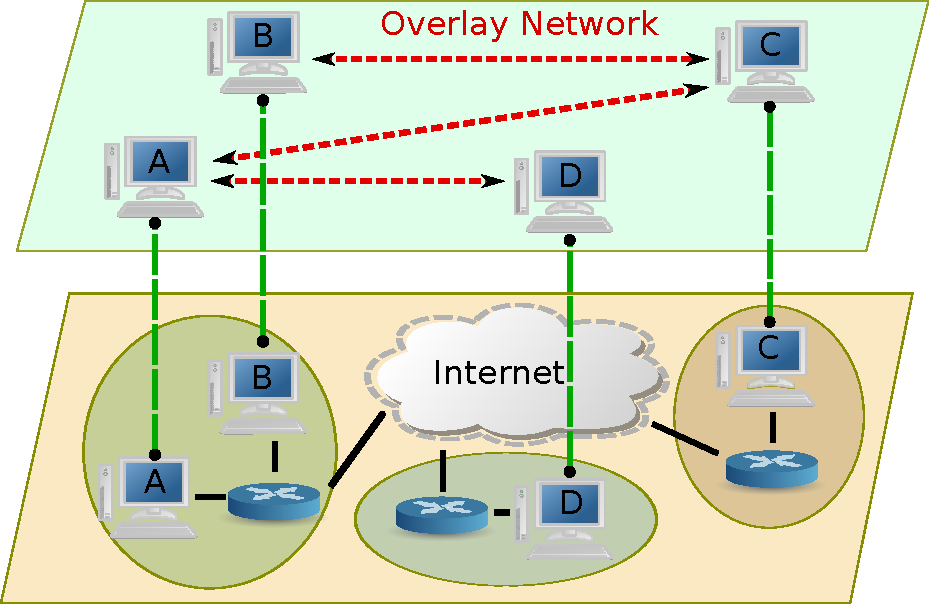
\includegraphics[scale=0.5]{img/p2p.pdf}
\caption{An example overlay network.}
\label{figure:overlay}
\end{figure}

An \emph{overlay network} is an abstract, logical interconnection of entities
formed on top of another network. It consists of a set of nodes, the computing
elements, that are being connected by virtual (logical) point-to-point links.
For example, the \emph{Asymmetric Digital Subscriber Line (ADSL)} is, actually,
an overlay network on top of the \emph{Public Switched Telephone Network
(PSTN)}. Figure \ref{figure:overlay} illustrates an example physical ethernet network
and the corresponding overlay network formed by four nodes. 
Nodes $A$ and $B$ are on the same local network, while $C$ and $D$ are in
different networks. The top layer represents the overlay network formed by these
nodes, which is a reflection of the application layer connections among these
nodes. As the topology of the network can change based on the application, in
this example, it is easy to observe that even though nodes $A$ and $B$ are in the same
network, their communication goes through node $C$ on another network,
demonstrating a non-optimal mapping between the physical and the overlay
networks.
An overlay network is generally useful when
abstraction of the network layer from the application layer is important for
applications, particularly when the underlying network structure is subject to
frequent changes.%, which is a common case for ad-hoc networks. 

The abstraction of overlay networks has been proposed as a way to implement
efficient, fully distributed, application layer services on top of a best-effort
IP layer forming a widely ranged family of protocols collectively known as
\emph{peer-to-peer} or \emph{p2p} for short. P2p network systems gained
significant attention, in recent years, due to their plethora of unique features
in supporting file sharing among huge numbers of (inter-) networked computers
called \emph{peers}, where each, such, \emph{peer} could act both as a resource
provider and a resource consumer. This changed the traditional
\emph{client-server} model dominating the internet and lead to the introduction
of the \emph{servent}-concept \cite{gnutella}, a portmanteau that blends the
notions of \emph{server} and \emph{client} to denote the twofold role of the
participants in a p2p network. Such serverless systems, proved to be able to
achieve outstanding aggregate resource capacities as participants join the
system
%\footnote{Unfortunatelly, there has been observed mitigation of this
%self-scaling property by the undesirable behaviour of participating users,
%usually answered in popular file-sharing systems; from \emph{free-riding} (i.e.
%in Napster and Gnutella networks \cite{saroiu_measurefileshare_2002,
%adar_gnutellafreeriders_2000, hughes_gnutellafreeride_2005}), to the
%distribution of illegal content and/or other \emph{socio-technical} issues
%\cite{hughes_socp2p_2008}.}, 
without requiring additional expenditure for infrastructure.


As p2p systems evolved, three main architectures have been emerged, namely:
\begin{itemize}
  \item \emph{centralized}
  \item \emph{decentralized unstructured}
  \item \emph{decentralized structured}
\end{itemize}

\emph{Centralized} architectures were the first to recognize that requests for popular content need not be sent to a central server but instead could be handled by the many hosts that already posses the content. \emph{Napster}, for example, maintained a \emph{central index server} based on file lists provided by participating peers. The central index server was queried by the users and it returned pointers to the actual content. Thus, by centralizing search while distributing downloads, Napster achieved a highly functional design that was widely acknowledged, at the time, as ``the fastest growing Internet application ever''. This centralized search facility, though, renders this scheme not fully distributed and can be proven its ``Achilles' heel'' in terms of being a scalability bottleneck, a central point of failure and vulnerable to malicious acts (e.g. \emph{Denial-of-Service (DoS) attacks}).

The centralized approach has been eventually replaced by architectures that distributed both the search and the download capabilities. In these \emph{decentralized unstructured} architectures, file placement is random, which means there is no correlation with the network topology whatsoever \cite{yang_improvep2psearch_2002}. The most important properties of such systems are that they support inherent heterogeneity of peers, are highly resilient to peer failures, and incur low maintenance overhead at handling the dynamics of peer participation \cite{stutzbach_churn_2006}. In the literature, they are also known as \emph{broadcast-based} systems, because they use \emph{message flooding} among peers (i.e. Gnutella\cite{gnutella}) or among super-peers (i.e KaZaA\cite{kazaa}) to propagate queries. 
Even though the unstructured approach became highly popular among file sharing applications, they do have a certain disadvantage in locating rare objects due to the unstructured nature and the limitations of the flooding approach. 
%Each (super-) peer receiving a query decreases the incoming query message's lifetime which is measured in \emph{time-to-live (TTL)} hops, back-propagates its results, and  if the lifetime of the incoming message did not expired (TTL did not reach zero), it forwards the message to all its neighbours except from the one it receives it from.
% TODO: maybe enumerate applications of decentralized unstructured p2ps.

Recently, \emph{decentralized structured} schemes have been proposed in order to provide a self-organising infrastructure for large-scale p2p applications \cite{ratnasamy_can_2001,stoica_chord_2001,antony_pastry_2001,zhao_tapestry_2001,maymounkov_kademlia_2002}. They implement a \emph{Distributed Hash Table (DHT)} that maps objects to nodes through a deterministic mechanism. The main advantage of the DHT approach of decentralized structured p2p networks over decentralized unstructured ones, is that they provide a guaranteed bound on the number of overlay routing hops that have to be taken in order for an object to be located even in the case where only a single copy exists in the system. This is $O \left ( log n \right )$ compared to Gnutella, that requires $O \left ( n \right )$ to reliably locate a specific object.
% TODO: maybe enumerate applications of decentralized structured p2ps. (OceanStore, Far)

%{\sethlcolor{yellow}\hl{HA: Give the brief advantages and disadvantages of structured and unstructured
%approaches here!}}

% TODO: enumerate applications of overlay networks and p2p systems regardless of architecture
% UNDER CONSTRUCTION
% Q&A: Need more??
Initial efforts targeted on the implementation of one-to-many addressing schemes
that could replace \emph{IP multicast} in providing higher quality of streaming
media through \emph{quality of service (QoS)} guarantees. IP multicast as well
as other proposals such as \emph{IntServ} and \emph{DiffServ}
\cite{cisco_diffserv_2005} have not seen wide acceptance (yet?), largely because
they require changes to all routers of the network. On the other hand, an
overlay network can be incrementally deployed on end-systems running the overlay
protocol software, without cooperation from the ISPs. Academic research includes
\cite{chu_esm_2000,jannotti_overcast_2000,kwon_tag_2002} among others.  Overlay
networks were also implemented in order to back the routing of messages to
destinations whose address is not known in advance. This resulted in the
appearance of well known peer-to-peer protocols such as \cite{gnutella} and
\cite{maymounkov_kademlia_2002} widely used for digital content sharing among
their network nodes.  Other special purpose overlay networks include
\cite{anderson_ron_2001} for resilient routing; \cite{subramanian_overqos_2004}
for quality of service guarantees; and \cite{clarke_freenet_2001} for anonymity;
to name just a few.

The main focus of this paper is the topology mismatch problem, therefore the
available approaches in overlay networks are briefly summarized, and interested
readers are pointed to the available surveys on overlay networks
\cite{TheotokisS04,LuaCPSL05}.

%%%%%%%%%%%%%%%%%%%%%%%%%%%%%%%%%%%%%%%%%%%%%%%%%%%%%%%%%%%%%%%%%%%%%%%%%%%%%%%
% start
%TODO: Maybe this section should be reviewed or deleted or go to another section
%Studying the behaviour of the various peer-to-peer schemes \cite{matei_mapgnutella_2002, lv_randomwalks_2002, merugu_str2unstr_2003} showed that the ad-hoc network topology of unstructured overlay networks that preserve \emph{Power Law} and \emph{Small World} characteristics\footnote{Power Law describes the node degree while the Small World describes characteristics of path length and clustering coefficient. The clustering coefficient for a node $\upsilon$ in a graph $G = \left( V, E \right)$ is defined as the ratio of the existing connections between $\upsilon$'s neighbouring nodes to $\gamma \times \left( \gamma - 1 \right)$, where $\gamma$ is the number of neighbouring nodes of $\upsilon$. High cluster coefficient means that neighbouring nodes of any node $\upsilon$ likely connect one another.} \cite{faloutsos_powerlaw_1999, saroiu_measurefileshare_2002} offer a more promising approach. Particularly:
%\begin{itemize}
%  \item Peer-to-peer clients are extremely \emph{transient}. Unstructured systems can have high maintenance traffic in delivering messages, updating the mapping, discovering failures and replicating lost data or pointers, making them insufficient on highly volatile networks.
%  \item \emph{Keyword searches} versus \emph{exact-match queries}. In DHTs there is a tight control between the data placement and the topology of the network. For this reason it is hard to efficiently support partially matched queries while Gnutella and other similar systems effortlessly support keyword searches and other complex queries since the mechanism is realized locally, on a node-by-node basis.
%  \item Popular content is located at multiple peers and thus it is more likely for a flooding-based search to return results. DHTs, on the other hand, fit better in the systems which require ability to reliably locate content, even in the extreme case that only a single-copy exists in the network.
%\end{itemize}
% end
%%%%%%%%%%%%%%%%%%%%%%%%%%%%%%%%%%%%%%%%%%%%%%%%%%%%%%%%%%%%%%%%%%%%%%%%%%%%%%%

% TODO: how 
%For this reasons, efforts have been placed for optimizing the efficiency of decentralized unstructured peer-to-peer networks. Research mainly focuses on
%\begin{inparaenum}[\itshape i\upshape)]
%  \item reducing unnecessary, redundant communication traffic, and
%  \item exploiting physical locality to reduce communication response.
%\end{inparaenum}
%The goal can be achieved at, both, the application-level network as well as the underlying physical one. In the first case by refining the message relay techniques, while in the second one, by adaptively reconstructing the application network to map as well as possible to the the physical network.

%%%%%%%%%%%%%%%%%%%%%%%%%%%%%%%%%%%%%%%%%%%%%%%%%%%%%%%%%%%%%%%%%%%%%%%%%%%%%%%
\section{The Topology Mismatch Problem}

% TODO: Define the problem
% UNDER CONSTRUCTION
% Q&A is it too late??

%{\sethlcolor{yellow}\hl{ {\cite{hsiao_redblue_2009}} states that:
%Liu {\cite{liu_thancs_2008}}  concluded that more than 70 percent of communication
%paths in an unstructured overlay do not exploit the physical network topology
%(i.e., the Internet topology), resulting in a topology mismatch between the
%overlay and the underlying network.  } }

One of the major issues that defines the efficiency of the overlay network is
the mapping of the physical links and the overlay paths. Ideally, overlay
networks are expected to achieve an optimal mapping among the overlay paths and
the underlying physical links, and avoid the inefficient mapping that is shown
in Figure \ref{figure:overlay}. The problem of constructing an optimal overlay
is referred to as the \emph{topology mismatch problem}, and formally defined as
follows:

\begin{definition}
    Let $V = \{v_1, ..., v_n\}$ be a set of points denoting the network nodes,
    $\{v_i, v_j\} \in E$ be the set of unicast distances between nodes $v_i$ and
    $v_j$, $G=(V,E)$ be a complete distance graph over $V$. The topology
    mismatch problem is to construct a minimal spanning tree,  where 
    node degree is restricted to a constant ($k\geq 2$) by the bandwidth of each node $v_i$.
\end{definition}

Constructing degree constrained spanning tree is known to be NP-Hard
\cite{NPBOOK}, as well as the topology mismatch problem
\cite{chawathe_scattercast_2000}. 
 Moreover, the internet is an interesting environment
where end-to-end latencies demonstrate triangle inequality violations (TIVs),
which further complicates the problem.
These delay space TIV is a consequence of the Internet's structure and routing
policies and thus will remain a property of the Internet for the foreseeable
future \cite{zheng_irprtt_2005}. TIVs affect network coordinate
\cite{cox_vivaldi_2004,wong_meridian_2005} and positioning \cite{ng_gnp_2001}
and makes difficult the construction of delay aware overlays.  A number of
heuristic approaches have been proposed in an effort to finding an algorithm
that performs reasonably and consistently well.

A topology unaware overlay network is able to control the sequence of peers a
message traverses before reaching its destination, but it is completely unaware
of how the actual packets are switched at the underlying infrastructure along
the overlay path. For example, a single logical point-to-point link on the
overlay, most of the time, corresponds to multiple physical links in the
underlying layer. Additionally, a link in the underlying network often serves
the mapping of several overlay paths causing increase of the traffic on the
physical link, which is also called the link's
\emph{stress}\cite{chu_esm_2002}.  Furthermore, the stochastic behaviour of
peers randomly joining and leaving the peer-to-peer network all cause the
overlay to physical mapping to create such unnecessary, redundant maintenance
traffic that impacts the efficiency of the network in terms of average response
time. 

%{\sethlcolor{yellow}\hl{
%HA: Motivation to solve topology mismatch problem:
%
%Most of the traffic (find refs!! see Location aware topology matching paper
%introduction for refs [31][29]) in the internet today is generated by P2P
%networks. The inefficient use of the network resources by the P2P protocols,
%especially the problem known as topology mismatch problem, causes unnecessary
%traffic load and a heavy stress
%on the internet infrastructure in general, and effects other users of the
%internet than the P2P nodes.
%}}


\begin{figure}
\centering
  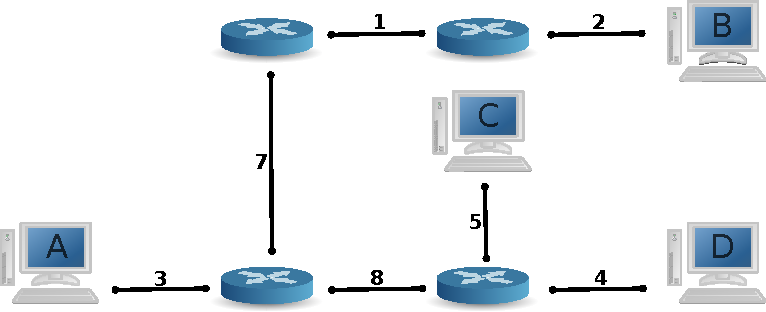
\includegraphics[scale=0.8]{img/phys.pdf}
\caption{Interconnection of nodes in the physical level.}
\label{figure:phys}
\end{figure}

\begin{figure}
\centering
  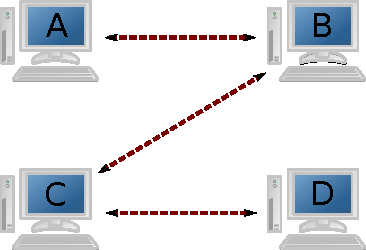
\includegraphics[scale=0.8]{img/over1.pdf}
  \hspace{3ex}
  \vline
  \hspace{3ex}
  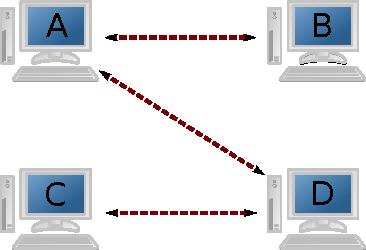
\includegraphics[scale=0.8]{img/over2.pdf}
\caption{HA: Put subfigure, and a new caption here}
\label{figure:over1}
\end{figure}

For example, assume nodes $A$, $B$, $C$ and $D$ are connected through the
physical network shown in Figure~\ref{figure:phys}, where the network costs are
given in milliseconds, and peer $A$ sends a message to peer $D$. If these peers
participate in an overlay network according to one of the setups of
Figures~\ref{figure:over1}~(left) and~\ref{figure:over1}~(right) then users will
yield different performances. In the first overlay shown in Figure
\ref{figure:over1}~(left), the message will traverse the following sequence of
links in the physical layer (marked with their costs): $3 \rightarrow 7
\rightarrow 1 \rightarrow 2 \rightarrow 2 \rightarrow 1 \rightarrow 7
\rightarrow 8 \rightarrow 5 \rightarrow 5 \rightarrow 4$. In the second overlay
shown in Figure ~\ref{figure:over1}~(right), the path will be: $3 \rightarrow 8
\rightarrow 4$. The total cost of the first path is $45 ms$, while the second
only costs a mere $15 ms$. Therefore, we can conclude that the second overlay is
more congruent with the underlying physical network than the first one and thus
more efficient.

% TODO: Argue on the problem
% UNDER CONSTRUCTION
Early incarnations of the overlay protocols, however, did not make use of the optimal
mapping with the physical network topology. Early Gnutella protocol, though were
considered far from scalable \cite{ritter_gnucantscale_2001}, randomly choose
logical neighbours without knowledge of the underlying network, effectively
causing mismatch between physical and application-level topologies.
Additionally, queries may be flooded to multiple paths merging in one peer while
in such case one of the paths would have been enough. 
%Nevertheless, peers may
%forward the same message to each other before they receive the query messages
%from each other.

Similar problems are observed in decentralized structured schemes also.
Typically, node IDs are assigned \emph{randomly}, resulting in excellent load
balancing, scalability and robustness.  Unfortunately, this randomness has a
negative impact on the \emph{routing locality} of the network. This means that
even though the target node can be reached with logarithmic overlay hops, the
distance traveled in the physical underlying network, during the overlay routing
process, can be far from optimal.  The ratio of the physical distance, a query
travels through the overlay to an object, and the minimal distance to that
object (i.e. though IP) is known in the literature as \emph{stretch} or
\emph{Relative Delay Penalty (RDP)} \cite{chu_esm_2000}.

Studies on peer-to-peer traffic reveals the effect of the peer-to-peer traffic
on the overall internet.  Measurements
\cite{seroiu_analysiscds_2002,sen_analyzep2ptraffic_2004} on some popular
systems, such as FastTrack, Gnutella and DirectConnect have shown that the
peer-to-peer traffic contributes the largest portion of the overall Internet
traffic.  \cite{matei_mapgnutella_2002} showed that, even given that 95\% of any
two nodes are less than 7 hops away from each other, a flooding-based algorithm,
like the one used by Gnutella, can generate 330TB/month in a 50.000 node
network!  Therefore, the efficiency of the overlay networks has serious
consequences on the overall well-being of the modern internet. 

% TODO: Taxomize the approaches that have been proposed in the literature
% for unstructured and structured overlay networks
% UNDER CONSTRUCTION
% VERY IMPORTANT SECTION
%\section{Taxonomy}
%
%% TODO: Unstructured
%% UNDER CONSTRUCTION
%Several overlay protocols for dealing with the problems derived from the
%topology mismatch problem have been proposed in the literature. Each
%implementation has different goals but all share some common ground on the
%aspect of the network functionality they focus on, in order to achieve them. In
%this section, the general taxonomy used throughout this paper to categorize the
%algorithms based on their functionality is presented.  The brief description of
%each category and sub-category is stated below.
%
%{\sethlcolor{yellow}\hl{CITE this paper {\cite{liu_ltm_2004}}}}
%
%\subsection{Forwarding based}
%
%Forwarding based methodology is generally adapted by distributed unstructured
%overlay systems. In this approach, a peer selects only a subset of its
%neighbours to re-broadcast query messages. The selection is made using one or a
%combination of various statistical metrics. Examples of such metrics are the
%number of responses received by a neighbour or the connection latency of the
%link between the nodes, etc. The forwarding based approach enhances search
%efficiency but has also several drawbacks. First, the search scope is reduced
%drastically.  Expanding the search scope, on the other hand, is no easy task
%because the overhead of forming multicast trees is proportional to the multicast
%group size.  Second, forwarding based schemes do not consider dynamic joining
%and leaving of peers so they do not scale well on dynamic environments.
%
%\subsection{cache based} 
%
%Caching based protocols are effectively used to reduce traffic costs and response
%times. The caching policy varies depending on the way protocol handles the index and the
%content. Centralized P2P systems
%use central index servers, while local caching systems, such as KazaA, use super peers
%to cache indices in a distributed way. Content caching is also possible in P2P
%systems, where nodes cache the forwarded content for further retrievals.
%Although caching has the above mentioned advantages,  duplication
%of messages still exist, which limits the scalability of these approaches.
%Therefore, cache based approaches are analyzed in the following categories:
%  \begin{itemize}
%    \item \emph{data index caching},
%    \item \emph{content index caching},
%    \item \emph{centralized}, and
%    \item \emph{local}.
%  \end{itemize}
%
%\subsection{overlay optimization based} 
%
%The overlay optimization based protocols modify the topology of the P2P network
%using various techniques. These approaches include creating spanning trees using 
%connection graphs, creating cluster of physically close nodes, or using latency
%information to detect proximity. The brief description of each category is presented
%below:
%
%  \begin{itemize}
%    \item \emph{Spanning tree based}. These approaches construct of a rich graph
%    based on the network connections and build minimum spanning tree on the
%    graphs, causing large traffic overhead to the system
%    \cite{chu_esm_2000,chu_esm_2002}.
%
%    \item \emph{Cluster based}. These approaches select to link physically
%    closer nodes with each other, therefore shrink the search scope
%    significantly while mapping accuracy is not always guaranteed.
%
%    \item \emph{Minimum latency first}. Use of latency as a metric to calculate
%    distance among peers. They require global latency information
%    ``landmarks''\footnote{Measuring latency between peers and stable Internet
%    servers.}.
%
%  \end{itemize}
%
%
%% TODO: Structured
%% UNDER CONSTRUCTION
%\subsection{proximity based}
%Xu \textit{et al.} \cite{xu_globstate_2003} state that there are three ways generating proximity information
%\begin{itemize}
% \item Expanding Ring Search\\
%Expanding ring search can be of two forms. First it can utilize the multicast
%infrastructure in the underlying network in order to emit its messages.
%Unfortunately such infrastructures are not widely deployed thus the
%implementations of this way of generating proximity information is limited to
%blindly flooding the neighbourhood to obtain reasonable results.
%
% \item Heuristics\\
%Heuristics are used in order to reduce the blindness of the expanding ring
%search and make realizations more efficient and effective. Unfortunately a
%common problem of all heuristic approaches is the local minimum pitfall in which
%the search might be caught into.
%
% \item Landmark Binning\\
%Landmark clustering is based on the view that nodes with similar distances to a
%set of predefined well-known landmark nodes are pretty likely of being close to
%each other. But this approach has its weaknesses as well, such as the fact that
%is a rather coarse grained approximation, therefore not particularly well suited
%for differentiating nodes within close distance to each other.
%
%\end{itemize}
%
%Castro \textit{et al.} \cite{castro_proximitydht_2002,castro_topawareroute_2002} on
%the other hand, comment on the three basic approaches in exploiting proximity
%in DHT protocols suggested by Ratnasamy \textit{et al.} \cite{ratnasamy_openq_2002}.
%These are:
%
%\begin{itemize}
% \item Geographic Layout\\
%The node IDs are assigned in such a way that nodes close by in the physical
%network topology, be close in the node ID space as well. Implementations that
%work relatively well with this approach have been incorporated into CAN. Nodes
%measure the RTT between themselves and a set of landmarks in order to match the
%CAN space as much as possible to the physical one. Unfortunately, the approach
%requires well known landmark servers and for that matter is  not fully
%self-organizing which can further lead to imbalanced node distribution. On
%other DHTs, such as Chord or Pastry, another problem emerges.  To gain fault
%tolerant properties, these protocols, replicate key-value pairs on neighbouring
%(in the ID space) nodes. When a proximity-based node ID assignment has been
%used, the needed failure resilience is undermined by the fact that close by
%nodes are more likely to suffer collective failures.
%
% \item Proximity Routing\\
%Proximity routing does not require routing tables be built using any knowledge
%about network proximity. On the other hand it exploits such knowledge in order
%to choose the best next hop during routing a message. This approach 
%balances between choosing the node that will further progress the routing
%towards the destination and choosing the closest entry in the routing table, in
%terms of network proximity. Thus, it is relatively less effective than
%geographical layout when applied to CAN(-like) implementations. Moreover, the
%technique has been incorporated into a version of Chord (TODO: PChord |
%additionally check whether this is true) causing an increase on the overhead of
%node joins and the size as well as maintenance cost of finger tables.
%\cite{dabek_cfs_2001} proposes a server selection scheme for the Chord DHT, on
%the domain of proximity routing selection. In \emph{CFS}, each node predicts
%the entire lookup latency as a function of the total number of nodes and the
%average overlay next routing peer. The problem is that it is very difficult to
%have a clear picture on the total number of nodes and the average hop latency
%from the local. This leads to rough estimations that consequently decreases
%overall performance.
%
% \item Proximity Neighbour Selection\\
%Finally, the third approach, constructs the routing tables using proximity
%knowledge. Tapestry and Pastry's mechanisms of routing table
%maintenance try to minimize the distance to nodes appearing in a peer's routing
%table. Since routing is based on longest node ID prefix match, messages 
%are gradually forwarded to nearby nodes at each routing step.
%\cite{castro_proximityp2p_2002} argues on how Pastry exploits proximity
%neighbour selection in order to create a scheme that is (more) location-aware
%compared to the other well-known DHTs (CAN, Chord).
%
%\end{itemize}
%
%{\sethlcolor{yellow}\hl{
%HA: Possible criteria: based on which protocol (eg Gnutella, CAN etc), peer
%selection (topology selection, cluster, cache etc), supports dynamic update,
%runtimes}}
%%\textbf{Algorithm} & \textbf{Overlay structure} & \textbf{Forwarding} & \textbf{Cache} & \textbf{Overlay optimization} & \textbf{Proximity information} & \textbf{Base protocol} & \textbf{Dynamic update} & \textbf{Runtime} \\
%
%
%{\sethlcolor{yellow}\hl{
%HA: Possible criteria2: Overlay optimization structure, base protocol (eg
%Gnutella, CAN etc), dynamic update, runtimes, scalability}}
%
%{\sethlcolor{yellow}\hl{
%HA: maybe add also the year of publication, and see if there is a pattern in
%terms of the method and the year??}}



Having understood the nature of the problem that peer-to-peer architectures face,
Section \ref{sec:unstructured} and \ref{sec:structured} discuss the recent academic work that has been conducted
in the field. What follows does not claim
to be a thorough citation of all known protocols that are available out there,
but instead, a careful selection of those that left a distinctive fingerprint
contribution in the efforts of the research community to alleviate the topology
mismatch problem.

%{\sethlcolor{yellow}\hl{
%Create a theoretical section. This is an Approximation alg for Top-mis problem
%
%A Near-Optimal Algorithm Attacking
%the Topology Mismatch Problem
%in Unstructured Peer-to-Peer Networks
%}}

%%%%%%%%%%%%%%%%%%%%%%%%%%%%%%%%%%%%%%%%%%%%%%%%%%%%%%%%%%%%%%%%%%%%%%%%%%%%%%%
\section{Unstructured Decentralized Algorithms}\label{sec:unstructured}

In this section, the unstructured decentralized P2P algorithms are analysed based on their architecture and
base methodology to tackle the topology mismatch problem. The
unstructured decentralized algorithms are visited and categorized based on their
use of the overlay structure, messaging between nodes, and on the techniques
proposed to detect proximity to optimize the topology. 
The base methods that unstructured P2P algorithms use to tackle the topology
mismatch problem can be categorized as Broadcast, Cache, Overlay Optimization, 
and Landmark Based. In this section, these methodologies are discussed in
detail and the algorithms in each category are highlighted.

%{\sethlcolor{yellow}\hl{
%HA: TALK ABOUT GNUTELLA HERE!!!!}}

\subsection{Broadcast Based}

In the naive Gnutella protocol, each received query request is forwarded to all the
neighbours, which clearly generates unnecessary traffic over the network. The
algorithms categorized in the \textit{broadcast based} methodology prefers
re-broadcasting the query messages to a selected subset of their neighbours,
where the selection criteria varies between algorithms.
The selection is made using one or a
combination of various statistical metrics, such as the reliability or the latency
of the link between nodes, etc.
The forwarding based approach enhances search
efficiency but has also the drawbacks of having drastically reduced search scope
due to the selective re-broadcasting policy, and scalability problems on large
P2P networks.
%Expanding the search scope, on the other hand, is no easy task
%because the overhead of forming multicast trees is proportional to the multicast group size.  
%forwarding based schemes do not consider dynamic joining
%and leaving of peers so they do not scale well on dynamic environments.

The forwarding based P2P algorithms and their details are presented below.

\paragraph*{\bf Improving search in peer-to-peer networks}

\cite{yang_improvep2psearch_2002} proposes an easy to implement and practical
solution to the inefficiency problem caused by blind flooding in Gnutella like
P2P file sharing protocols. The paper replaces blind flooding with three
approaches, namely \textit{iterative deepening}, \textit{directed BFS}, and
\textit{local indices}. In \textit{iterative deepening}, the search is performed
on a BFS tree with multiple preset depths. The depth limit is iteratively
increased by the source node for each query based on the quality of the results.
The source node, after examining the results, may issue a new request by
increasing the depth limit, which will trigger the nodes at the last depth
level to resume the search. The iterative approach avoids to start the search
from scratch at each iteration and reduces the load of the nodes on the upper
levels of the tree. The major drawback of \textit{iterative deepening} is the
delay between successive iterations, as the source node needs to examine the
results at each iteration before deciding to quit or resume the query.  The
\textit{directed BFS} tries to avoid this delay by forwarding the query messages
only to a selected set of neighbours, in which the selection criteria varies
from the number of results received previously, distance in terms of hops,
bandwidth, or the query load of the neighbour. In \textit{local indices}, each
node sustains a local data index of the nodes within a radius of $r$ hops of
itself and uses this local index to remotely query the neighbour nodes without
generating additional traffic.  \textit{Local indices} greatly reduces the
aggregate bandwidth usage of the network and improves query efficiency, however,
updating the indices in cases with frequent node joins and leaves introduces a
serious overhead to the system if the radius is kept broad.

\paragraph*{\bf Gia}

\emph{Gia} \cite{chawathe_gia_2003} is an effort to solve the scalability
problem of the unstructured P2P file sharing systems, in particular Gnutella.
The main novelty in the design of Gia is the replacement of blind flooding
approach of Gnutella with random walks \cite{lv_randomwalks_2002}. Although
random walks is a step in the right direction, issuing only a single copy of the
query within the network reduces the search scope, thus affects the success rate
of the query.  In order to overcome this limitation, Gia introduces a
token-based flow control algorithm, which is essentially an intelligent flow
control algorithm that gradually redirects the queries to nodes with more chance
of answering. Gia also acknowledges the heterogenity in peer bandwidth,
processing power, disk speed, etc, of the nodes in P2P networks and uses this
heterogenity when connecting nodes to each other, such that by using a topology
adaptation algorithm, Gia ensures that high capacity nodes have high degrees and
low capacity nodes are within short proximity of high capacity nodes. In order
to prevent overloading of nodes with query requests, Gia uses a token-based flow
control algorithm in which each node announces the number of query requests it
can handle in terms of tokens to its neighbours, so that neighbours only forward
query requests to nodes that they previously received tokens from. Although the
topology adaptation algorithm Gia uses improves the scalability of the network,
it does not help much in solving the topology mismatch problem, since it does
not consider the underlying physical topology.

\paragraph*{\bf Distributed Cycle Minimization Protocol}

The flooding based query approach of Gnutella creates many duplicate packets in
the network. Nodes receive the same query request from various neighbours, which
they generally discard when identified as duplicate. One other reason for
duplicate messages is the cycles in the forwarding paths. These duplicate
packets affect the performance of the P2P network negatively by increasing the
overall resource usage. Moreover, the more active nodes, that have high
capacity, high bandwidth, or contribute more to the network, suffer more from
the overhead caused by the duplicate packets. Therefore, \emph{Distributed Cycle
Minimization Protocol (DCMP)} \cite{zhu_dcmp_2008} is introduced as a method to
remove the cycles and eliminate the duplicate packets, without sacrificing the
connectivity. In DCMP, once a cycle is detected, the most powerful node in the
cycle is elected as the \emph{Gate Peer} and the cycle is cut from a special
link such that the distance of all the nodes within the cycle to the \emph{Gate
Peer} is minimized. The process is managed by using two special message types,
\emph{Information Collection (IC)} and \emph{Cut Message (CM)}. One disadvantage
of DCMP is that since the distance a forwarded message can travel is limited
with the TTL value, which is practically $7$ in Gnutella, the DCMP cannot detect
cycles of length larger than $7$. Even though cycle elimination improves the
network performance, it does not solve the topology mismatch problem.


%\subsection{Cache Based}
%
%Caching based protocols are effectively used to reduce traffic costs and response
%times. The caching policy varies depending on the way protocol handles the index and the
%content. Centralized P2P systems
%use central index servers, while local caching systems, such as KazaA, use super peers
%to cache indices in a distributed way. Content caching is also possible in P2P
%systems, where nodes cache the forwarded content for further retrievals.
%Although caching has the above mentioned advantages,  duplication
%of messages still exist, which limits the scalability of these approaches.
%Therefore, cache based approaches are analyzed in the following categories:
%  \begin{itemize}
%    \item \emph{data index caching},
%    \item \emph{content index caching},
%    \item \emph{centralized}, and
%    \item \emph{local}.
%  \end{itemize}
%

\subsection{Cache Based}
Caching is a widely used methodology to exploit the locality to minimize the
redundant transfer of data, which is successfully used in web servers and file servers.
As peers in a P2P system also work as servers, intuitively it is expected that
P2P file sharing systems can also benefit from caching. However, one of the most
important characteristic properties of P2P systems is that nodes
join and leave frequently, and the lifetime of a query is relatively short
compared to web servers, which makes caching in P2P networks nontrivial. There are
usually two levels of caching possible in file sharing systems, the indices or
pointers to data can be cached, or the data itself can be cached. Caching is
already implemented and successfully used in some commercial P2P systems. One
popular example is KazaA, which uses caching of indices in its super peers.
We present the other protocols that use caching and their details below.

\paragraph*{\bf Replication Strategies in Unstructured Peer-to-Peer Networks}

\cite{Cohen02} aim to improve the inefficient blind search algorithm by
replicating the data in a peer to peer network. The main intuition behind the
idea of replication, or using cached copies, is that as the number of copies for
each item increases in the network, it would be easier for a search algorithm,
even a random one, to locate these items. In order to analyse the feasibility of
such replication approach, the authors investigate three different replication
strategies, namely uniform, proportional, and square root allocation. In the
uniform model, the copies of items are uniformly replicated in the network,
while in the proportional model, the items are replicated based on their query
rate, so that frequently queried items are replicated more. The square root
allocation is a strategy proposed by the authors, which is a model between the
uniform and proportional allocation.  In order to evaluate the outcomes of the
replication models, the authors compare the overall costs of successful and
unsuccessful searches in the network. The results can be summarized as follows;
the uniform allocation model minimizes the maximum search size, therefore
reduces the time spent on an unsuccessful search. The proportional model, on
the other hand, promotes the more frequently queried items by replicating them
more, therefore decreases the search time for popular items, but suffers when
locating the rare items. The authors also claim that the expected successful
search size is the same for uniform and proportional models, and any approach
between them would behave much better. Therefore they propose the square root
allocation approach, which is a replication strategy that minimizes the expected
search size of successful queries in P2P networks.

\paragraph*{\bf Tracing a large-scale Peer to Peer System: an hour in the life of
Gnutella}

\cite{Markatos02} analysis the network traces of the Gnutella network and
detects that query requests in Gnutella has locality, and proposes a caching
algorithm that exploits this locality. The analysis of the trace data reveals
other important facts about the structure of the Gnutella network and the query
data.  One significant observation is that the geographic locations of clients
do not have a correlation with the number of query requests they receive. This
is an obvious result of the topology mismatch problem caused by the overlay
structure of the Gnutella network. Gnutella traffic is observed to be bursty
both for query requests and query responses, even in longer intervals, and nine
out of ten queries do not generate any response due to the inefficient design of
the Gnutella network. When developing a caching system to exploit locality,
applying an approach similar to web caching does not fit well with P2P systems.
The caches in P2P systems not only have to consider the query string, but also
the TTL value, the source of the query, and the time of the query as well.  In
general, even though optimum caching is hard to achieve, it is reported that
caching improves the overall performance of the Gnutella system.

\subsection{Overlay Optimization Based}

The overlay optimization based protocols modify the topology of the P2P network
using various techniques. The two commonly used approach that is investigated in
this section are creating spanning trees using 
connection graphs, and creating cluster of physically close nodes. 
%The brief description of each category is presented below:
Spanning tree based approaches construct rich graphs based on the network
connections and build minimum spanning trees on the graphs. Even though the
spanning tree provides efficient query performance, the construction
and the update costs of the spanning tree, especially in dynamic environments
with many nodes joining and leaving the network, cause large traffic
overhead to the system \cite{chu_esm_2000,chu_esm_2002}.

The cluster based approaches on the other hand select to link physically closer
nodes with each other, therefore shrink the search scope significantly. However,
commonly used methods for determining the correct physical positions of nodes
over the internet does not always return reliable results, therefore mapping
accuracy is not always guaranteed.

Below, the details of the algorithms that use the spanning tree based or cluster
based topology optimization methods are presented.

\paragraph*{\bf Narada}

Narada \cite{chu_esm_2000,chu_esm_2001,chu_esm_2002} is a generic protocol to
design self adapting overlay networks, that can achieve application layer
multicast without requiring IP multicast at the network layer. Although Narada
is not originally designed as a peer-to-peer file sharing application protocol,
it has become one of the pioneering works in the overlay networks area.  Even
though the design of the IP multicast protocol is finalized a while ago, and
some of the routers on the internet today already support this protocol, the IP
multicast idea did not take off as anticipated. One of the main reasons for this
delay is that the IP multicast violates the stateless design of the current
internet. Although the multicast is not widely used, and the future of the
protocol is not bright, there are multiple applications that need this kind of
service, such as IP TVs, P2P networks, streaming services, etc. The application
layer multicast is then a valid alternative for these applications.  The authors
claim that, although Narada is not as efficient as IP multicast, still it
provides reasonable performance, without the additional cost of implementing
multicast services on the current internet infrastructure. The main reason for
the inefficiency is due to the Topology mismatch problem.  Narada tries to solve
this problem by building a richer connected graph\footnote{ENarada
\cite{li_enarada_2008} used Gossip protocol for the construction}, called a
mesh, and building per source minimum spanning trees.  Narada also maintains the
graph and the trees dynamically updated on node joins and leaves. Moreover, Narada tries
to optimize the physical link stress, the overall resource usage and the
relative delay among end systems. The main limitation of Narada is that although
it works reasonably well for small groups, it does not scale well for larger
networks, therefore it is not suitable for P2P file sharing applications which
can easily scale to millions of nodes.


\paragraph*{\bf Adaptive Overlay Topology Optimization and Adaptive Connection
Establishment}

\emph{Adaptive Overlay Topology Optimization (AOTO)} \cite{liu_auto_2003} is one
of the first attempts, along with Narada, from the P2P research community to
address the topology mismatch problem. AOTO is a distributed algorithm
that uses \emph{Selective Flooding} and \emph{Active Topology} to optimize the
overlay network topology. The \emph{Selective Flooding} algorithm creates a minimum
spanning tree over the overlay and uses this tree instead of
flooding the whole network, without shrinking the search scope. 
In \emph{Active Topology}, the physical locations of nodes are estimated based
on the network delay among them and physically close nodes are connected as
neighbours to revise the overlay topology as close as possible to the physical
network topology. Overall, AOTO reports a $55\%$ performance improvement in
terms of the traffic load. In \emph{Adaptive Connection Establishment (ACE)}
\cite{liu_ace_2004}, the authors extend the idea by introducing optimizations
based on the depths of the minimum spanning trees. As the network delay is not always a reliable estimation
method to detect physical locations of the nodes, the algorithm still suffers
from the discrepancies caused by mislocated nodes.

\paragraph*{\bf Location-aware Topology Matching}

Peer-to-peer algorithms designed without considering the topology mismatch
problem generates unnecessary heavy traffic on the internet infrastructure, due
to the popular use of these P2P programs for file sharing. \emph{Location-aware
topology matching (LTM)} \cite{liu_ltm_2004} proposes a method to
optimize the overlay structure of the P2P network based on the physical
topology. In doing so, LTM issues a special message called
\textit{TTL2-detector} to detect the latency of $N^2$ neighbours around each
node. The latency information gathered is later used to evolve the overlay
network into a more efficient one, without reducing the search scope. Each node
examines the latency information with the neighbours and low productive
connections are dropped and replaced by more efficient ones, thus reducing the
latency on the overall network, and eliminating some potential inefficiencies,
such as unnecessary crossing of messages over autonomous system (AS) boundaries, etc. Although the
LTM approach improves the overall efficiency of the P2P network, since it uses
the latency to detect close by nodes, does not use the real physical topology
information, therefore does not offer a guaranteed bound to the
topology mismatch problem.

\paragraph*{\bf Scalable Bipartite Overlay}

\emph{Scalable Bipartite Overlay (SBO)}
\cite{liu_bipartite_IPDPS,liu_bipartite_2007} improves the overhead of creating
and maintaining a minimum spanning tree cost by randomly dividing the nodes into
two groups, red and white, and assigning different tasks to different groups.
The white peers measure distances to neighbours by using the network delay as
the metric and reports the results to red peers. The red peers, equipped with the
information of all two hop ($N^2$) neighbours, creates a minimum spanning tree
of these neighbours and assigns efficient forwarding paths. The white peers can
further optimize their positions within the overlay if need be.

%\paragraph*{\textbf{Two-Hop-Away Neighbour Comparison and Selection\\}}
%
%\paragraph{}
%Work in \cite{liu_thancs_2005,liu_thancs_2008} proposes a distributed heuristic called \emph{Two-Hop-Away Neighbour Comparison and Selection (THANCS)} that
%\begin{inparaenum}[\itshape i\upshape)]
%  \item is completely distributed and needs no global knowledge,
%  \item presents trivial overhead compared to the query cost savings
%  \item its convergent speed of the algorithm is fast enough (faster than minimum spanning tree approaches) so that is effective to dynamic environments, and
%  \item does not shrink the search scope.
%\end{inparaenum}
%
%\paragraph{}
%THANCS is considered a \emph{local search method}, in the sense that it targets in finding a locally optimum solution, by exploiting knowledge within a 2-hop radius. The algorithm consists of two main components: \emph{piggybacking neighbour distance on queries} and \emph{neighbour comparison and selection} which are furtherly discussed bellow.
%
%\paragraph{Piggybacking neighbour distance on queries}
%Using network delay as a metric for measuring the distance, each peer probes distances with its immediate naighbours and stores information locally. For this reason a special query message type, \emph{Piggy Message (PM)}, is introduced. It is 6 bytes long and includes two fields: Neighbour IP Address and Neighbour Distance. A peer $P$ constructs a PM for its neighbour $Q$, which contains $Q$'s IP address and $Q$'s distance from $P$. When $P$ receives a query from $Q$, this PM will be piggybacked by the query that goes to all other neighbours of peer $P$. Upon receiving such a query message, each of the other neighbours will detach the PM, record the $PQ$ distance and process the query. This PM will not be further forwarded. In selecting which incoming queries  should piggyback a PM the paper proposes the \emph{pure propability-based (PPB)} and the \emph{new neighbour triggered (NNT)} policies.
%
%\paragraph{Neighbour comparison and selection}
%Figure~\ref{figure:thancs} illustrates this component of the THANCS algorithm. A peer $S$ probes the distance to all known unprobed $N^2(S)$\footnote{$N^2(S)$ denotes the set of peers being two hops away from $S$, while $N(S)$ denotes the set of direct logical neighbours of $S$.}. The distance of $SP$ is known to $S$. Upon receiving a PM from node $P$ with the distance of $PQ$, $S$ follows one of the following:
%\begin{itemize}
%  \item $Q \in \left( N(S) \cap N^2(S) \right)$, i.e. $Q$ is direct neighbour of $S$. In this case $S$ will compare cost of $SQ$, $SP$ and $PQ$. If the most costly connection is one of $SQ$ or $SP$ the corresponding link will be put into a \emph{will-cut list}\footnote{Links are not immediately disconnected when put in the will-cut list. There are useless for forwarding but are kept active, for some time, in order to serve query responses that are traveling to the source peer along the inverse search path.}. If the most costly connection is $PQ$ then $S$ will do nothing, as the fully distributed nature of the algorithm will give a chance to either $P$ or $Q$ to cut the connection.
%  \item $Q \in \left( N^2(S) - N(S) \right)$, i.e. $Q$ is a two-hop-away neighbour of $S$. If $S$ hasn't probed $Q$ before\footnote{A distance cache is maintained and looked up in such a case.}, it probes and stores the result in the \emph{distance cache}. Having the distance of $SQ$, $S$ compares costs of $SQ$, $SP$ and $PQ$. If $SQ$ is the most costly, $S$ will not establish the connection. If $SP$ is the most costly, $S$ will establish connection $SQ$ and put $SP$ in the will-cut list. If $PQ$ is the longest, $S$ will keep  the connection with both $P$ and $Q$, expecting that $P$ or $Q$ will eventually disconnect link $PQ$, later.
%\end{itemize}
%
%\begin{figure}
%\centering
%  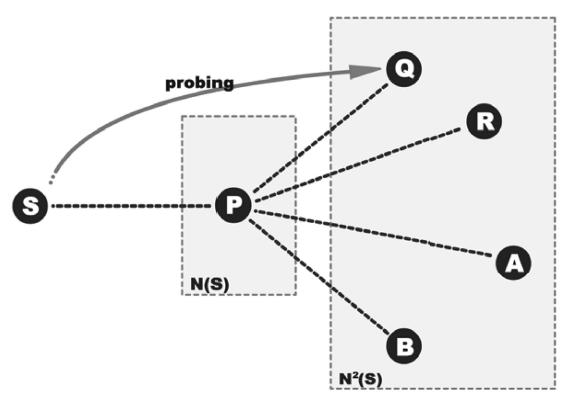
\includegraphics[scale=0.4]{img/thancs.jpeg}
%\caption{Probing two-hop-away neighbours}
%\label{figure:thancs}
%\end{figure}
%
%\paragraph{}
%In a static environment THANCS has been proven to be effective; optimizing 45 percent out of the 60 percent of mismatched paths, constructing a nearly optimal overlay. This leads to a 60 percent reduction in traffic cost as well as a 40 percent decrease in query response time. In dynamic environments (Gnutella 0.6/Limewire super-peer-like and Ion flat-like), THANCS saves up to 70 percent of the traffic cost in the super-peer topology and 55 percent for the flat one. Average response time is also decreased by 60 and 45 percent, respectively. Generally, THANCS has similar performance to LTM, without needing synchronization. SBO, incurring half the  overhead of AOTO, reduces the traffic cost the most, while THANCS has lower response time and converges faster than SBO. THANCS is, thus, more suitable for a more dynamic environment. In addition, THANCS is easy to implement and its operation overhead is trivial, compared with the other three approaches. This design, however, has the limitation of not being easily extend to also support non-flooding-based systems.


\paragraph*{\bf Peer-exchange Routing Optimization Protocols}

\cite{qiu_prop_2007} introduces two protocols called Peer-exchange Routing
Optimization Protocols (PROP) to adjust the neighbourhood graph of the overlay
network in order to reduce the overall link latency of the network. The PROP
algorithms are based on the exchange of neighbours among peers, which is
triggered by the mutual benefit of both peers to reduce the network delay.  In
PROP-G (Generic), peers exchange all their neighbours with another peer, while
in PROP-O (Optimized) only selected number of neighbours are exchanged among
peers. The PROP-G is a generic protocol that guarantees the connectivity of the
overlay graph during exchanges, therefore can be applied to both unstructured
and structured overlay networks. 


\paragraph*{\bf T2MC}

T2MC \cite{shi_t2mc_2008} uses traceroute logs to detect the AS boundaries and
cluster close by peers with each other to reduce the redundant multiple message
passes between the AS boundaries. T2MC uses a customized k-mean classification
algorithm with $k=2$ to perform the classification, and exploits the stable
structure of the internet routers to guide clustering.
Even though traceroute provides detailed information about the network
structure, use of traceroute creates overhead to the overall network structure.
For this same reason, it is not unusual for network administrators to disable
this support on their network routers, which may affect the performance of the
T2MC algorithm. 

%\paragraph*{\textbf{T2MC\\}}

%\paragraph{}
%\emph{T2MC}\cite{shi_t2mc_2008} exploits some properties of the Internet paradigm and clusters nodes belonging to the same ISP without any centralised control or predefined system parameterization. The algorithm considers the dynamic nature of peers and exploits the stable nature of routers in order to build a topology location relationship among end peers.
%
%\paragraph{}
%Some special routers split the physical network into autonomous system domains. Using a Traceroute mechanism T2MC searches for latency leaps among the path to a host in order to form ``near'' and ``remote'' router clusters. This is achieved by a 2-Means Classification, defined by the following steps:
%\begin{enumerate}
% \item the peer chooses the minimum and maximum Latency results from the Traceroute for initializing the cntroinds of two sets ``first'' and ``second''.
% \item The peer calculates, for all hops allong its tracerouted path, the absolute distance to the centroids of both sets and assigns the routers to that centroid with which it has the smaller absolute distance.
% \item The peer calculates the latncy mean and variance value of two sets
% \item If the variance is larger than a predefined threshold then the algorithm takes a loop from step 2 picking the two latency mean values as new centroids of sets ``first'' and ``second''.
%\end{enumerate}
%Ultimately peer will end up with two sets having the minimum intra-set variance. Finally the peer chooses the router from ``second'' set with the minimum hops attribute and sets it as a threshold. The selected router and all others whose hops attribute is larger than the threshold are classified as ``remote'' router cluster. The remaining are classified as ``near''. From the ``near'' class, the peer chooses the one with maximum hops attribute as its edge router, and registers it along with the all the ``near'' cluster into the DHT of the p2p overlay. As new peers join the network, those that share the same edge router or any of the members of the ``near'' router clustersm ther would gather to form a ``close'' peer cluster. As Edge routers can provide more valuable information than other members of the ``near'' set, T2MC was designed to prioritize interaction of peers and edge gateways.
%
%% TODO: figure t2mc.jpeg (a) stars represent edge routers (b) hop leaps
%
%\paragraph{}
%The use of Traceroute as a tool for implementing the distance measuring infrastructure raise concearns about its efficiency and scalability. Being, primarilly, a network diagnostic utility, it is concearned too heavy weighted and intrucive for use in a larger scale\cite{ratnasamy_binning_2002}. Additionally, disabling ICMP is a common administrative policy for edge sites to enforce security, while dumping BGP routing tables\cite{krishnamurthy_bgpclust_2000} is not directly available to the application layer.

\paragraph*{\textbf{Unnamed Unstructured!!\\}}
% TODO: to be reviewed

\paragraph{}
In \cite{hsiao_redblue_2009}, Hsiao et al, claim to construct topology-aware unstructured overlays that \emph{guarantee} performance qualities in terms of
\begin{inparaenum}[\itshape i\upshape)]
  \item the expected communication latency among any two overlay peers regardless of the network size, and
  \item the broadcasting scope of each participating peer.
\end{inparaenum}

The algorithm constructs an undirected graph $G = \left( V, E \right)$ comprised by two subgraphs. The first, namely $G^{\left( red \right)} = \left( V^{\left( red \right)}, E^{\left( red \right)} \right)$ in the paper's context, includes all vertices of $G$ and ensures the connectivity of the graph by securing at least one path between any two nodes. In contrast, $G^{\left( blue \right)} = \left( V^{\left( blue \right)}, E^{\left( blue \right)} \right)$, contains those vertices of $G$ that have free edges to link to other nodes and because these are fully utilized, the following also stands $E = E^{\left( red \right)} \cup E^{\left( blue \right)}$.

A joining peer $u$, partitions its neighbours into two subsets, the $B_u^{\left( red \right)}$ and $B_u^{\left( blue \right)}$. In order to populate the $B_u^{\left( red \right)}$ subset, peer $u$ samples peers uniformly and at random. Then, each of these selected peers discovers a routing path starting from itself towards the node with the smallest (or the largest) ID in the system.

\paragraph*{\bf Distributed Domain Name Order}

%{\sethlcolor{yellow}\hl{HA:  In paper/introduction nice advantages of unstructured networks:
%
%Unstructured P2P networks o?er a number of
%important advantages: (i) An unstructured network
%imposes very small demands on individual nodes,
%and more speci?cally it allows nodes to join or leave
%the network without signi?cantly a?ecting the sys-
%tem performance. (ii) Unstructured networks are
%appropriate for content-based retrieval (e.g., key-
%word searches) as opposed to object identi?er loca-
%tion of structured overlays. (iii) Finally unstructured
%networks can easily accommodate nodes of vary-
%ing power. Consequently, they scale to very large
%sizes and they o?er more robust performance in
%the presence of node failures and connection
%unreliability.
%}}

\emph{Distributed Domain Name Order (DDNO)} \cite{zeinalipour-yazti_ddno_2005}
uses the domain names to detect topologically close nodes based on the
assumption that nodes within the same domain are topologically close to each
other. Half of the possible connections of a node is used to connect to these
local peers, and the other half is used to randomly connect to the peers
anywhere on the network.  \textit{DDNO} is a heuristic approach to solve the
topology mismatch problem, with local connections to improve the efficiency and
reduce the delay on the network.  The random connections on the other hand help
ensure the connectivity in the network and avoid partitioning. \textit{DDNO}
uses \textit{Split-Hash} and \textit{dnMatch} algorithms to detect locality by
using domain names.

\subsection{Landmark Based Proximity}\label{sec:landmark}

Detecting the proximity of a node using landmarks, also known as \textit{Landmark
Clustering}, is based on the view that nodes with similar distances to a
set of predefined well-known landmark nodes are pretty likely of being close to
each other. But this approach has its weaknesses as well, such as the fact that
is a rather coarse grained approximation, therefore not particularly well suited
for detecting the correct positions of nodes within close distance to each other.

\paragraph*{\bf Landmark Binning}\label{sec:landmark_binning}

Landmark Binning \cite{ratnasamy_binning_2002} is an approach to partition close
by nodes into bins based on their distance to well known anchor nodes within the
internet. In order to detect locality, nodes use network latency (round trip
time) as a measurement technique. The network latency, even though not always
accurate, is selected in this work because its non-intrusive, transparent and
easy to apply structure. In order for the binning to work, authors assume that
there are a few well known anchor servers with known physical locations on the
internet. The authors estimate that around 12 servers will do the job. The nodes
measure their distance to all these servers and record the latency values for
each. Later, the tuple of these latency values represents the bin of each node.
Nodes with similar latency values are assumed to be close to each other, or at
least within the same AS. The landmark binning is designed as a generic model
that can work both on structured and unstructured P2P networks, and
\cite{ratnasamy_binning_2002} has the detailed description of the algorithm for
both topologies. As the main operation of the algorithm is independent from the
underlying model, and does not change for structured and unstructured networks,
we classify and give the details of the algorithm in this decentralized
unstructured section, and omit the duplicate work in the decentralized
structured section. The landmark binning is also proposed as a good candidate to
work on content distribution networks. The major disadvantage of landmark
binning is to install and maintain landmark servers on different AS, all over
the world.  A typical P2P network usually has a couple of million nodes
connected at any time, which introduces possible scalability problems in terms
of the landmark servers.  The authors claim that latency estimation does not use
much network resources and in order to avoid the possible scalability problems
the authors propose to replace single landmark servers with clusters of servers
within the same physical area. However, this approach does not reduce the
possible high network traffic flow through these landmark servers. One other
possible problem is the incorrect binning caused by inaccuracy in delay
measurements methods, as the network latency is not a proven accurate method for
location estimation.


\paragraph*{\bf mOverlay}
mOverlay \cite{zhang_moverlay_2004} addresses the scalability problems that
affect static landmark servers by introducing the dynamic landmarks. The
nodes are divided into groups based on their distances to these groups and the
neighbour nodes in these groups behave as dynamic landmarks. The mOverlay
protocol is composed of two main parts, initially adding a new node to the
overlay by selecting the closest group, and maintaining the overlay afterwards.
Finding the correct closest group is the most important part of the overlay
construction. The authors also formally prove that any new node can reach its
group by performing at most $O(logN)$ communications within the network.

\renewcommand\arraystretch{1.4}% (MyValue=1.0 is for standard)

%\begin{figure}[h!]
\hspace{-3ex}
\begin{center}
\footnotesize
%\begin{tabular}{
\begin{landscape}
\begin{longtable}{
|>{\columncolor[gray]{.7}}m{0.1\columnwidth}
|>{\columncolor[gray]{.9}}m{0.1\columnwidth}
|>{\columncolor[gray]{.9}}m{0.2\columnwidth}
|>{\columncolor[gray]{.8}}m{0.1\columnwidth}
|>{\columncolor[gray]{.9}}m{0.1\columnwidth}
|>{\columncolor[gray]{.8}}m{0.1\columnwidth}
|>{\columncolor[gray]{.9}}m{0.1\columnwidth}
|>{\columncolor[gray]{.8}}m{0.1\columnwidth}
|}
\caption{Decentralized Unstructured Algorithms} \label{fig:unstruct_compare_table} \\
\hline
\rowcolor[gray]{.5}
\textbf{Algorithm} & \textbf{Arch.} & \textbf{Overlay structure} & \textbf{Base protocol} &
\textbf{Dynamic update} & \textbf{Runtime} & \textbf{Scalability} & \textbf{cites}\\
\hline
\endfirsthead
\multicolumn{4}{c}%
{\tablename\ \thetable\ -- \textit{Continued from previous page}} \\
\hline
\rowcolor[gray]{.5}
\textbf{Algorithm} & \textbf{Arch.} & \textbf{Overlay structure} & \textbf{Base protocol} &
\textbf{Dynamic update} & \textbf{Runtime} & \textbf{Scalability} & \textbf{cites}\\
\hline
\endhead
\hline \multicolumn{4}{r}{\textit{Continued on next page}} \\
\endfoot
\hline
\endlastfoot
\textbf{Narada} & Decentralized unstructured & \textbf{Overlay optimization
based}. Creates a mesh (richer connected graph) and builds minimum spanning
trees on this mesh & & Yes. Supports incremental evolving & & Small and sparse
groups & 2000  \\

\hline
\textbf{Gia} & Decentralized unstructured & \textbf{Forwarding based} Replaces
Gnutella flooding with random walk, and introduces KaZaA style supernodes. Uses
dynamic topology adaptation protocol &
 Gnutella & Yes & & Better than Gnutella & 974  \\

\hline
\textbf{Adaptive Overlay Topology Optimization} & Decentralized unstructured & \textbf{Overlay optimization
based}. Creates overlay multicast tree with Selective Flooding protocol&
Gnutella & Yes, using Active Topology protocol & & Better than Gnutella & 36 \\

\hline
\textbf{Location-aware Topology Matching} & Decentralized unstructured &
\textbf{Overlay Optimization Based}. Uses \textit{TTL2-detector flooding}, \textit{low productive
connection cutting}, and \textit{source peer probing}. & Gnutella & Yes & & Better than Gnutella & 204 \\

\hline
\textbf{Replication Strategies in Unstructured P2P Networks} & Decentralized unstructured &
\textbf{Cache Based}. Uses uniform, proportional and square root allocation
strategies to replicate data. & Gnutella & Yes & & Better than Gnutella & 580 \\

\hline
\textbf{Tracing a large-scale Peer to Peer System: an hour in the life of Gnutella.} & Decentralized unstructured &
\textbf{Cache Based}. Proposes a caching algorithm based on the traces of the Gnutella traffic & Gnutella &
Yes & & Better than Gnutella & 199 \\

\hline
\textbf{Improving search in P2P networks} & Decentralized unstructured &
\textbf{Forwarding Based}. Uses \textit{iterative deepening}, \textit{directed
BFS}, and \textit{local indices} to improve efficiency. & Gnutella & Yes & & Better than Gnutella & 380 \\

\hline
\textbf{Distributed Cycle Minimization Protocol} & Decentralized unstructured &
\textbf{Forwarding based} Uses a decentralized cycle elimination protocol  &  & Yes &  &  & 9 \\

\hline
\textbf{Scalable Bipartite Overlay} & Decentralized unstructured &
\textbf{Overlay optimization based} Uses bipartite partition graph and builds
local minimum spanning trees  & Gnutella & Yes &  & Better than Gnutella & 77 \\

\hline
\textbf{Adaptive Connection Establishment} & Decentralized unstructured &
\textbf{Overlay optimization based} Forms Neighbour Cost Tables, builds local
minimum spanning trees and perform local optimizations & Adaptive Overlay
Topology Optimization (AOTO), Gnutella & Yes &  & Better than Gnutella & 110 \\

\hline
\textbf{Hops Adaptive Neighbour Discovery} &  &
 &  &  &  &  & 1 \\

\hline
\textbf{Two-Hop-Away Neighbour Comparison and Selection (THANCS)} & Decentralized unstructured &
\textbf{Overlay optimization based} Uses piggybacking to discover neighbour
distances and selects neighbours  & Gnutella & Yes &  &  & 36 \\

\hline
\textbf{mOverlay} & Decentralized unstructured &
\textbf{Overlay optimization based} Uses dynamic landmarks to find node locality
& & Yes &  & Due to dynamic landmarks and grouping, more scalable than tree-based or mesh-based protocols & 123 \\

\hline
\textbf{Distributed Domain Name Order (DDNO)} & Decentralized unstructured &
\textbf{Overlay optimization based} Connects half of the nodes connections to
the nodes in the same domain and the other half to random nodes, therefore
supports locality and topological connection  & & Yes &  & Yes, by using super
peers & 5 \\

\hline
\textbf{Peer-exchange Routing Optimization Protocols} & Works with both decentralized
structured and unstructured &
\textbf{Overlay optimization based} Optimizes overlay by the exchange of
neighbors among peers  & & Yes &  & Yes & 13 \\

\hline
\textbf{MAY OMIT- T2MC} & Decentralized unstructured &
\textbf{Cluster based---{\sethlcolor{yellow}\hl{ IS IT ALSO PROXIMITY BASED?}}} Uses traceroute results for clustering the
nodes  & &  &  &  & 1 \\

\hline
\textbf{Unnamed-unstructured} & Decentralized unstructured &
\textbf{Overlay optimization based} Minimizes the communication delay and
maximizes the broadcasting range & & Yes &  & Better than THANCS and mOverlay & 7\\

\hline
\textbf{Landmark Binning} & Can work with both decentralized structured and unstructured &
\textbf{Proximity based, landmark binning} Uses network latency to partition
nodes into bins & & Yes &  &  & 817 \\

\hline
%\end{tabular}
\end{longtable}
\end{landscape}
\end{center}
\vspace{-2.5ex}
\vspace{-2.5ex}
%\end{figure}

\subsection{Discussion on Unstructured Decentralized Algorithms}

Earlier in section \ref{sec:unstructured} we presented the state of the art unstructured
decentralized P2P algorithms in four different categories based on their
architecture; broadcast based, cache based, overlay optimization based, and
landmark based. In this section, we present a final discussion of all the
methods including the advantages, disadvantages,
and novelties presented in order to tackle the topology mismatch problem.
Table \ref{fig:unstruct_compare_table} presents an overview of all the
unstructured decentralized algorithms described earlier in this section.

The broadcast based approaches in general propose intelligent neighbour
selection algorithms in order to replace the inefficient blind
flooding algorithm of Gnutella.
Instead of forwarding the queries to all the neighbours, intelligently selecting
neighbours with high probability of answering the query, or neighbours that have
some specific features such as high bandwidth, high capacity, or low latency in
practice reduces the aggregate resource usage of the P2P network and improves
the overall performance of the system. However, since the broadcast based algorithms
proposed do not consider the underlying physical topology when selecting the
neighbours, or optimizing the overlay structure, the algorithms do not offer a
solution to the topology mismatch problem. Although in practice the algorithms
work, none can guarantee that a single link is not used by more than necessary,
or the created topology resembles the underlying physical topology. Broadcast
based methods can be used in conjunction with other approaches to improve the
quality of the P2P systems.

The success of caching, as a well studied method in the client server internet
applications, also made it a good candidate for the peer-to-peer networks. Even
though caching improves the performance, and reduces the overall resource usage
of P2P systems, the design of caches is non trivial compared to the web caching
systems. Due to the unique structure of the P2P overlays, each node being a
server and a client simultaneously, two important problems has to be solved when
designing caches. First, the lifetime of a query is short, as the nodes join and
leave frequently. Second, the result of a single query string is not always the
same, and changes based on the TTL value, source of the query, the lifetime of
the query, etc. So, in order to develop a successful caching system in P2P
systems, these parameters also have to be considered. Even though the state of
the art P2P algorithms using caching methods reduce the resource usage of the
network, since the physical network topology is not considered by any algorithm,
the proposed systems do not provide direct ways to overcome the topology
mismatch problem caused by the overlay network.

The overlay optimization based algorithms can be analyzed in
two main topics, the minimum spanning tree based ones, and the clustering based ones.
Even though the standardization of the IP multicast protocol is completed a
while ago, and some vendors deployed routers supporting the protocol, in
practice the standard is not widely embraced as predicted, mostly because the
protocol violates the stateless design of the internet routers. The research
community, as an alternative proposed application layer multicast frameworks,
such as Narada, to simulate the same multicast protocol without requiring IP
multicast services. The application layer multicast, however, is not as
efficient as IP multicast, and suffers from the topology mismatch problem.
Narada, and its followers (AOTO, LTM, SBO) try to solve the topology mismatch
problem by building a richer connected graph and forming minimum spanning trees
over this graph that can efficiently route messages among peers. The application
level multicast protocol, initiated by Narada, is a generic protocol that can be
applied to P2P file sharing, as well as content distribution networks. The
original Narada algorithm is designed for small groups therefore it is not
scalable. The followers try to solve the scalability problem by introducing
various methods including forming minimum spanning trees for each nodes' $N^2$
neighbours, partitioning the graph into two random groups where each group is
responsible of different tasks, or performing local optimizations dynamically on
the overlay graph. The advantage of the minimum spanning tree based approaches
is that they maintain the connectivity on the network in an efficient way, while
still not shrinking the search space. However, building and maintaining a
minimum spanning tree creates a huge overhead for the network. 
One other popular approach used in overlay optimization is the cluster based
approaches. In cluster based approach, nodes use various methods to detect
physically close nodes to form clusters. T2MC uses traceroute logs and DDNO uses
domain names to cluster close by nodes. However, the accuracy of the methods
used to form clusters directly affect the success rate of the algorithm. Traceroute for
example is a heavy weight protocol to frequently use on the network, and most of
the network vendors for this reason do not allow traceroute calls. The major problem with
cluster based approaches is that the limited connectivity within the local
domains shrink the search scope dramatically, which negatively affects the
search performance of the P2P system. DDNO addresses this limitation by allowing
half of each nodes connections to be to random nodes over the network, which
balances the efficiency of the clustering approach with improved connectivity.

In landmark based proximity method, nodes use network delay (round trip
time) as a distance measurement method to position themselves based on distance
measurements to apriori known servers on the internet. The servers behave as
landmark points, and nodes use an estimation method to discover their positions.
The landmark servers are either used by nodes to directly calculate their
positions, or indirectly used to cluster nodes into groups or bins based on
their estimated distances to well known landmark servers, due to the assumption
that nodes with similar distances to a set of landmarks are physically close to
each other over the network. The landmark based protocol has two important
drawbacks. Firstly the network delay is not a reliable distance estimation
method. For example, based on the load on the network the delay to certain
nodes or networks can change from time to time, which will eventually affect the
distance measurements and wrong measurements will lead to wrong estimated positions for the
nodes, or incorrect and non optimal clusterings of the nodes. The second drawback of
using landmark servers is the cost of installing and maintaining many landmark servers over the internet
for various AS domains. As popular P2P file sharing applications usually have
millions of peers connected at any time, it is not false to assume that the hardware and the network costs of
maintaining these landmark servers will be quite high. 
A possible solution to the scalability problem of the static landmark servers is to use ordinary nodes as dynamic
landmarks once they estimate their own positions. Even though this approach scales
much better than static landmark servers, still the measurement accuracy problem affects
the overall performance of the system.


\section{Structured Decentralized Algorithms}\label{sec:structured}

In this section, the algorithms proposed for the structured decentralized
architectures are analysed and categorized based on their use of the proximity
information to optimize the underlying structure. In structured P2P algorithms,
the construction of the routing tables among nodes determines the efficiency of
the algorithms.  Therefore, routing tables that represent the underlying
physical structure well can achieve much better performance. For this reason,
the proposed methods for topology mismatch problem generally use different
levels of proximity information to optimize the routing table close to the
physical network. We analyze the structured decentralized algorithms based on
the categories presented in
\cite{castro_proximitydht_2002,castro_topawareroute_2002,ratnasamy_openq_2002}.
In this section, the details of the methodologies used and the algorithms for
each methodology are discussed in details.

%{\sethlcolor{yellow}\hl{HA:  Talk about Tapestry, Pastry, CAN and Chord briefly here!}} 

\subsection{Geographic Layout}

Geographic layout is used as a method to optimize the routing table of the
structured algorithms to represent the physical network topology as close as
possible. In this method, physically close nodes are detected, and they are
positioned closely in the overlay structure. In order for this method to work,
there should be means to detect physical proximity of internet nodes. One
popular method is to use the well known internet servers, or servers dedicated
for this sole purpose, as landmark nodes, similarly as discussed previously in
Section \ref{sec:landmark} (\textit{Landmark Based Proximity}).  The inaccuracy in
the positioning using landmarks, and the cost of deploying and maintaining these
landmarks are the major disadvantages of these systems. Even though managing the
overlay structure based on the geographic layout of the nodes improves the query
efficiency of the system, on the other hand, it tends to create hotspots, and
the needed failure resilience is undermined by the fact that close by nodes are
more likely to suffer collective failures.

\paragraph*{\bf Global Soft-State}

\textit{Global Soft-State} \cite{xu_globstate_2003} builds a global map to help
choose shorter routing paths, combining the landmark binning method and small
scale distance probes to reveal the proximity properties of the underlying
network to the overlay. This global view of the state is made available to all
nodes in order to help them find the best way to route their messages.
\textit{Global Soft-State} operates in two main stages, generation and using of
the proximity information. For generating the proximity information a hybrid
approach is proposed, which uses landmark clustering as a preprocessing step in
order to select a number of potential nearest neighbour candidates and then
refine the selection by incorporating an RTT scheme to ultimately choose the
closest node. For using the proximity information, the algorithm chooses a
different path from the classic gossiping approaches for constructing and
maintaining the overlay. It is based on landmark clustering based strategic
placement of proximity information on the overlay enabling any node to access
such information using a landmark number that reflects its physical position in
the network. For various logical regions\footnote{This might be a high-order
zone in the eCAN\cite{xu_ecan_2002} context or a set of nodes sharing a
particular prefix in overlays such as Pastry.} maps of physical information are
built and published where each node may appear in a maximum of $log\left( N
\right)$ such maps. To dynamically adapt to changing network conditions, a node
subscribes to relevant \emph{soft states} that utilize a notification system in
order to initialize any necessary neighbour re-selection.

Maintaining several host states at different layers, makes any content migration
costly. Additionally, the method does not make any continuing effort to remap the
overlay structure after a node successfully joins, in order to adapt its state to
any occurrence of condition change. Although this approach greatly reduces the
routing latency to far nodes, it is unable to dynamically identify nodes that are
close to routers and gateways in order to construct the secondary overlay.
Nevertheless, static recognition of such nodes is currently done based on BGP
reports and pre-chosen landmarks, sacrificing the self-organising attribute of
traditional DHTs.

\paragraph*{\bf Mithos}

\textit{Mithos} \cite{waldvogel_mythos_2003} is a P2P protocol which
incorporates a directed incremental probing to find near optimal node placement,
and classified by its authors as an integration of geographic layout
and proximity routing overlay optimization methods.

The bootstrap phase of \textit{Mithos} starts with a subset of existing members
as the first set of candidates, and while the iteratively closest nodes are
detected by probing the neighborhood, the candidate neighbor list is updated. In
order to avoid a local minima \textit{Mithos} probes all the neighbours within a
two hop distance from the current minimum before concluding the process.

After finding its first neighbour, the newcomming peer is assigned an ID using
information gathered during the iterative neighbour selection phase. Virtual
coordinates are assigned to the newcomming peer by using the distances of two
closest nodes and their neighbours, so that Euclidean distances between the node
and all known hosts predict the network latency between
them\cite{cox_vivaldi_2004}.  The benefit of these synthetic coordinates are
that they are explicitly used as the node's ID, and distance computations among
nodes can be done in ID space without requiring physical measurements.

The last step of the algorithm is the interconnection among neighbours.
\emph{Mithos} uses a \emph{quadrant}-based mechanism according to which each
node establishes a link to the closest neighbour in each quadrant. During
forwarding, the next hop is performed towards a neighbour in the same quadrant
as the final destination. The newcoming node may not know of other neighbours
in all quadrants, therefore, the node first identifies neighbours in all
quadrants using a mechanism based on ideas similar to a perimeter
walk\footnote{Used in Greedy Perimeter Stateless Routing (GPSR) protocol.} and
then improves the results using parallel path processing by taking into account
further geometric properties of node relationships.

One major limitation of \textit{Mithos} is that the protocol cannot handle
dynamic arrivals and removals from the network, as is happens in mobile
networks.

\paragraph*{\bf LAPTOP}

\textit{LAPTOP} \cite{wu_laptop_2007},  organises the overlay into a tree based
hierarchy with main focus on reducing hops during message routing as well as
minimizing maintenance overhead. Additionally, a caching scheme is also
incorporated so as to further reduce routing table update costs. The authors
theoretically show that in \textit{LAPTOP} routing path length is bounded by $O(log_d
N)$ and node joining and leaving in the overlay network is bounded by $O\left( d
log_d N \right)$ hops in a balanced overlay tree, where $N$ is the number of
nodes, and $d$ is the maximum degree of each node. \textit{LAPTOP} implements
the geographical layout approach  and constructs a geographical layout in a
self-organizing and efficient fashion, by estimating the round trip time (RTT)
to a small number of nodes in the overlay network in order to make them roughly
aware of their physical distances among them.

Each node is assigned an address in a dotted format (e.g 1.3.4). Each octet
ranges from $1$ to $d$, where $d$ is the maximum degree of the nodes. The
assignment process is done by appending a unique octet to the address of each
nodes
parent, while root node is assigned address 1.  The routing scheme is similar to the
longest-prefix IP matching scheme. At each forwarding hop, any message travels
up the tree until the first common ancestor of source and destination node is
reached and then starts descending to arrive to its target. During tree
traversals, special entries in the routing tables, called \emph{routing cache},
are maintained in order to increase routing efficiency and achieve finer load
balance. Caching enables a node to forward a message to a better longest-prefix
match than that of its direct ancestor making a large, quicker and more cost
effective step through the overlay and toward the destination. To improve
scalability, the number of children nodes and the size of the routing cache are
limited.  In terms of overlay maintenance, \textit{LAPTOP} incorporates a simple
\emph{heartbeat}-based technique where each parent node is responsible for
monitoring its children.  At join process the newcomming node is assigned its
level label as well as its address by its parent node. Additionally it
initializes its routing table (with normal and caching entries) as it traverses
the overlay in search for its parents node.  During a graceful departure, the
referred node checks for children in the overlay. If it does not have any, it
simply notifies its parent and leaves. If it has, it selects the child node with
the lowest RTT to it in order to take its place so that the locality property is
preserved.

\subsection{Proximity Routing}
Proximity routing does not require routing tables to be built using any knowledge
about network proximity. On the other hand it exploits such knowledge in order
to choose the best next hop during routing a message. This approach 
balances between choosing the node that will further progress the routing
towards the destination and choosing the closest entry in the routing table, in
terms of network proximity. Thus, it is relatively less effective than
geographical layout when applied to CAN(-like) implementations. Moreover, the
technique has been incorporated into a version of Chord causing an increase on the overhead of
node joins and the size as well as maintenance cost of finger tables.
%
%\cite{dabek_cfs_2001} proposes a server selection scheme for the Chord DHT, on
%the domain of proximity routing selection. In \emph{CFS}, each node predicts
%the entire lookup latency as a function of the total number of nodes and the
%average overlay next routing peer. The problem is that it is very difficult to
%have a clear picture on the total number of nodes and the average hop latency
%from the local. This leads to rough estimations that consequently decreases
%overall performance.
%
The methods that use proximity routing and their details are listed below.

\paragraph*{\bf Proximity in Kademlia}
Before discussing {\em Proximity in Kademlia}, it would be helpful to briefly
summarize the highlights about the {\em Kademlia} protocol.
{\em Kademlia} \cite{maymounkov_kademlia_2002} is a distributed hash table (DHT) based
protocol for P2P networks, which uses an iteration based lookup algorithm. The
protocol uses the standard $160$ bit ID system for nodes and locates the nodes in
a prefix binary tree, where IDs are used as prefixes. The iterative lookup
operations are done over this prefix binary tree, which converges to logarithmic lookup
times. The ID's are assigned randomly, therefore in Kademlia,
there is no proximity control, which results in inefficient use of the underlying
network during lookup and retrieve operations.

{\em Proximity in Kademlia} \cite{kaune_pkad_2008} introduces proximity controls
over the base Kademlia protocol to optimize the underlying network usage of the
protocol. The authors define an abstract {\em underlay metric} that calculates
the suitability of establishing a communication link between peers as a cost
function, based on the used proximity criteria (RTT, ISP locality, etc.).
{\em Proximity in Kademlia} adapted both {\em proximity routing} and {\em
proximity neighbour selection} overlay optimization algorithms for controlling proximity. Therefore,
we categorize the protocol only in this section, and skip the discussion in the
further {\em proximity neighbour selection} section (Sec.\ref{sec:pns}). {\em
Proximity in Kademlia} also uses the MaxMind GeoIP database\footnote{MaxMind
Geolocation Technology. http://www.maxmind.com} to detect the
proximity information of a given peer based on its region, country, or ISP
location, and use this information to form clusters of nearby peers. One
other method {\em Proximity in Kademlia} uses is the Vivaldi \cite{cox_vivaldi_2004} protocol. However, authors report that
clustering approach performs better than Vivaldi protocol based on their
experiments. Authors also report that {\em Proximity routing} protocol
successfully worked with the Kademlia protocol and improved the locality of the
connections over peers.

\paragraph*{\bf CHOord considering Proximity on IPv6 (CHOP6)}

\textit{CHOP6} \cite{morimoto_chop6_2007} is designed based on the
\textit{Chord} protocol. \textit{CHOP6} roughly estimates the proximity among
nodes by exploiting the IPv6 address format and RTT information if available.
The proximity estimation is achieved by introducing a 64-bit ID scheme in which
the least significant bit part is the IPv6 global routing prefix and thus
enabling a longest prefix match scheme. The protocol is designed based on the
observation that it is possible to estimate a node's geographical location by
simply examining the upper 32-bits of its IPv6 address. Moreover, similar to
\textit{Chord}, \textit{CHOP6} uses a finger table, whose entries hold more than
one candidate node.  

\paragraph*{\bf Chord6}
\emph{Chord6} \cite{xiong_chord6_2005} is another \textit{Chord} variant that
tries to exploit the hierarchical features of IPv6 in order to create a
substrate that reduces interdomain traffic between service providers.
\textit{Chord6} is based on the original Chord protocol, and the main difference
from the original protocol is in the identifier definition. Therefore, the
approach can be easily portable to other DHTs such as CAN, Pastry and Tapestry.
In Chord6 the identifier contains two parts: the higher bits are obtained by
hashing the node's IPv6 address prefix of specific length, while the remaining
lower bits are the hash value of the rest of that IPv6 address. As a result of
this assignment, nodes in a domain will be mapped onto a continuous key space on
the overlay network, which avoids unnecessary message forwarding across
different service providers, thus minimizing overall routing cost. 


\subsection{Proximity Neighbour Selection}\label{sec:pns}
\textit{Proximity Neighbour Selection} constructs the routing tables using proximity
knowledge. The proximity information used in this method is different than the
landmark based systems described in the \textit{Geographic Layout} section, as TTL values between
nodes, or directly node ID prefixes are used to detect proximity.  Tapestry,
Pastry, and CAN successfully implemented the proximity into their algorithms by
using this approach.  The routing protocol in Pastry is based on longest node ID
prefix matching, while CAN uses RTT values to detect close by nodes.
\cite{castro_proximityp2p_2002}  reports that proximity neighbour selection as
an effective proximity based method.
%
Proximity Neighbor Selection based algorithms are described in detail below.


\paragraph*{\bf DHT-PNS}

Chord-DHT-PNS \cite{hancong_pnsbased_2006} implements proximity neighbour
selection on top of the Chord DHT. The main purpose is to use proximity
information to group physically close by nodes as neighbours in the DHT table.
In order to detect proximity, virtual network coordinates of peers are used, by
using the Vivaldi protocol \cite{cox_vivaldi_2004}. The virtual coordinates are
then used by the nodes to map to identifier space in the DHT. The space is
partitioned using a \emph{concentric circle clustering scheme} where successive
cycles of radiuses $\rho$, $2\rho$, $3\rho$ and so on, are constructed. Then the
formed annuluses are divided into $2\chi-1$ \emph{sectors}, where $\chi$ denotes
the sequence number of the annulus starting from $\chi = 1$ for the centre
cycle. It is proved in the paper, that this way each sector occupies the same
area as does the center cycle. Assuming uniform node distribution, this
characteristic, favours a more load balanced clustering operation. Every sector
in this $2D$ coordinate space is mapped to a unique \emph{region} in the DHT
space forming a multi-layer node identifier space.  Thus, any nodes that belong
to the same sector, are mapped to the same region as well, preserving their
proximity relationship unveiled by the use of the Vivaldi protocol. The
individual pieces are mapped to the identifier space uniquely, allowing
logarithmic lookup operations with high probability on Chord.

\paragraph*{\bf IP-based Clustering (IPBC)}
Proximity neighbour selection algorithms use probing and other measures
to detect proximity. However, such methods are either are not precise enough, or
creates overload in the network. \emph{IP-based clustering}
\cite{karwaczynski_ipbc_2007} is a proximity neighbour selection based
algorithm in which the authors propose to use the IP address prefixes (16 bit
for IPv4) in order to detect proximity.  \cite{freedman_iploc_2005} states that
$97\%$ of prefixes larger than $24$ bits belong to a single geographical
location. However, using less number of bits creates less precise results and
more number of bits increase the burden on the network and reduce the possible
number of neighbours. Therefore, a careful selection is required in terms of
performance/accuracy tradeoff. The {\em IP-based Clustering} generates a key and
its prefix and stores its prefix in the DHT itself, so that any newly joining
nodes with the same IP prefix can query the prefix and identify all the
neighbours with the same prefix relatively easily. Nodes periodically update
their entries in the DHT and remove their entry when they leave, or the entry is
timed out with no further activity detected from the node.


\paragraph*{\bf Cone}

\textit{Cone}\cite{wang_cone_2007} extends the Chord using proximity neighbour selection
topology optimization algorithm. The proximity information is generated using
landmarks and RTT based distances to landmarks.  \textit{Cone} uses a two-layered
identifier space. The first, named Chord-layer identifier, denoted as
$Id_{Chord}$, is the same as in Chord. The second is the Cone-layer
identifier, $Id_{Cone}$ which is constructed by two component identifiers. The
first, known as \emph{group identifier (gid)} denotes a relevant group the node
belongs to while the second, namely \emph{local identifier (lid)} indicates the
local identifier within the group. The group concept, which is introduced here,
is a way of dividing nodes according to a common $Id_{Chord}$ prefix.  The
structure of a Cone overlay, retains the Chord's circular topology. The difference
lies on the fact that, now, two rings are created. A big ring, where nodes with
the same \emph{gid} are arranged at each position. Each of these positions are a
smaller ring for the particular group's \emph{lid}s. The routing is achieved in
both clockwise and counter-clockwise directions in the big-ring, for which two
routing tables are maintained, namely \emph{front} and \emph{back} finger
tables. Entries in these tables, display physical network
proximity with the current node. Moreover, a third table called \emph{group}
table maintains information about other online peers within the current node's
group in a way that entries are now close in the ID space.

\paragraph*{\bf SAT-Match: Self-Adaptive Topology Matching}

\textit{SAT-Match} \cite{ren_satmatch_2004} is a protocol that specifically
tries to solve the topology mismatch problem by mapping the overlay network as
close as possible to the physical one. Even though no theoretical proof is
given, valid results are obtained and demonstrated through experimentations.
Similar to the other approaches in the proximity neighbour selection,
\textit{SAT-Match} uses probing to detect close by peers and obtain proximity
information. However, as an additional feature, \textit{SAT-Match} peers can do
selective jumps to adjust their locations in the DHT, if it reduces the stretch
of its one-hop neighbourhood. The stretch is defined as the ratio between the
average logical and physical latency of a link. It is reported that, due to the
selective jumps, the \textit{SAT-Match} achieves $40\%$ reduction in link
stretch, and when used with the \textit{Landmark Binning} approach (see Sec.
\ref{sec:landmark_binning}), the reduction rate increases up to $60\%$.
For dynamic environments, with frequent node arrival and leave,
\textit{SAT-Match} scales much better than \textit{Mithos}, due to its self
adaptation mechanism and selective jumps.

\emph{SAT-Match} uses a small TTL value for the probing messages in order to
reduce redundancy\cite{jiang_lightflood_2008}. This process begins as soon as
the node joins the network using a DHT mechanism. Each probing message contains
information about the source and a small TTL value. The recipient of such a
message returns information about itself to the source and forwards the probing
message to its neighbours if the TTL is non-zero. The discovered nodes are
referred to as $TTL-k$ neighbourhood of the source node based on the $TTL$ distance
to the source node. 

Blindly selecting the peer with the smallest RTT as neighbour is, generally, not
the optimal decision to make in order to achieve global \emph{stretch} reduction.
In a structured scheme, when a node jumps to connect to a
physically close node, it may need to connect to other distant nodes to maintain
the structure's integrity, thus creating an overall increase in the overlay's
\emph{stretch}. The two nodes with the smallest RTT is then used in order to
select one zone to jump in this phase. The algorithm is as follows: The source
node $S$ calculates the stretch change of its $TTL-1$ neighbourhood and that of
the $TTL-1$ neighbourhood of the first of the previously selected peers. These
calculations are made as if the jump has been made. If the stretch reduction is
over a predefined threshold the jump is performed, otherwise the second selected
candidate is picked and the same computations are performed. If again, the
threshold is not met, then no jump is ultimately done. In case of a jump, this
is performed as a combination of \emph{leave} and \emph{join} operations, in the
CAN context.



%\begin{figure}[h!]
\hspace{-3ex}
\begin{center}
\footnotesize
\begin{landscape}
\begin{longtable}{
|>{\columncolor[gray]{.7}}m{0.1\columnwidth}
|>{\columncolor[gray]{.9}}m{0.1\columnwidth}
|>{\columncolor[gray]{.9}}m{0.2\columnwidth}
|>{\columncolor[gray]{.8}}m{0.1\columnwidth}
|>{\columncolor[gray]{.9}}m{0.1\columnwidth}
|>{\columncolor[gray]{.8}}m{0.1\columnwidth}
|>{\columncolor[gray]{.9}}m{0.1\columnwidth}
|>{\columncolor[gray]{.8}}m{0.1\columnwidth}
|}
\caption{Decentralized Structured Algorithms}\label{fig:struct_compare_table}\\
\hline
\rowcolor[gray]{.5}
\textbf{Algorithm} & \textbf{Arch.} & \textbf{Overlay structure} & \textbf{Base protocol} &
\textbf{Dynamic update} & \textbf{Runtime} & \textbf{Scalability} & \textbf{cites}\\
\hline
\endfirsthead
\multicolumn{4}{c}%
{\tablename\ \thetable\ -- \textit{Continued from previous page}} \\
\hline
\rowcolor[gray]{.5}
\textbf{Algorithm} & \textbf{Arch.} & \textbf{Overlay structure} & \textbf{Base protocol} &
\textbf{Dynamic update} & \textbf{Runtime} & \textbf{Scalability} & \textbf{cites}\\
\hline
\endhead
\hline \multicolumn{4}{r}{\textit{Continued on next page}} \\
\endfoot
\hline
\endlastfoot

\hline
\textbf{Global Softstate} & decentralized structured &
\textbf{Proximity based, landmark clustering} Uses first landmark clustering
then measures RTTs to identify close nodes & & Yes &  &  & 195 \\

\hline
\textbf{Mithos} & decentralized structured &
\textbf{Proximity based} Uses nodes as topology landmarks and directed
incremental probing to optimize topology & & Yes &  & Scales well as all
operations are local ??? & 172 \\

\hline
\textbf{Self-Adaptive Topology Matching} & decentralized structured &
\textbf{Proximity based} Uses lightweight probing and
selective jumps to optimize the topology & CAN & Yes &  & Better than Mithos
& 40 \\

\hline
\textbf{Delay Aware P2P System} & &
\textbf{} & &  &  &  & 1 \\

\hline
\textbf{VERSION OF CHORD - DHT-PNS} & decentralized structured &
\textbf{Proximity based} Uses Proximity Neighbour Selection and the Vivaldi
system & Chord  & Yes &  &  & 5 \\

\hline
\textbf{MAY OMIT- VERSION OF CHORD - Quasi-Chord} & decentralized structured &
\textbf{Proximity based}  & Chord  & Yes &  &  & 0 \\

\hline
\textbf{LAPTOP} & decentralized structured &
\textbf{Geographic layout based} Hierarchical overlay structure  &   & Yes &  & routing path length $\log{_d N}$, 
join/leave overhead $d\log{_d N}$& 4 \\

\hline
\textbf{IP-Based Clustering} & decentralized structured &
\textbf{Proximity based} Proximity neighbour selection based on longest common
prefix of IP addresses &   & Yes &  &  & 1 \\

\hline
\textbf{CHOord considering Proximity on IPv6} & decentralized structured &
\textbf{Proximity based} Uses IPv6 address format to provide proximity &  Chord
& Yes &  & Better than Chord & 1 \\

\hline
\textbf{Proximity in Kademlia} & decentralized structured &
\textbf{Proximity based} Applies  proximity neighbour selection (PNS) and proximity route selection (PRS)
to Kademlia & Kademlia & Yes &  &  & 13 \\

\hline
\textbf{Cone} & decentralized structured &
\textbf{Proximity based} Uses proximity neighbour selection (PNS) & Chord & Yes
&  & Better than Chord & 3 \\

\hline
\textbf{Dynamo} &  & &  & 
&  & & 3 \\

\hline
\textbf{MAY OMIT-BADLY WRITTEN-PChord} & decentralized structured &
\textbf{Proximity based}  &  Chord
& Yes &  & & 16 \\

\hline
\textbf{AChord} & &  &  
&  &  & & 7 \\

\hline
\textbf{Chord6} & decentralized structured &
\textbf{Proximity based} Uses IPv6 hierarchical address format to cluster
topologically close nodes & Chord & Yes
&  &  & 14 \\

\hline
\end{longtable}
\end{landscape}
\end{center}
\vspace{-2.5ex}
\vspace{-2.5ex}
%\label{fig:struct_compare_table}
%\end{figure}


\subsection{Discussion on Structured Decentralized Algorithms}

In section \ref{sec:structured},  we presented the state of the art structured
decentralized P2P algorithms in three different categories based on their
handling of the network structure to tackle the topology mismatch problem:
geographic layout based, proximity routing based, and proximity neighbour
selection based. In this section, we present a final discussion of all the
methods including the advantages, disadvantages,
and novelties related to solve the topology mismatch problem.
Table \ref{fig:struct_compare_table} presents an overview of all the
structured decentralized algorithms described earlier in this section.

Structured P2P network algorithms use a global distributed hash table or a
prefix tree structure to uniquely lookup peers or their data in the overlay
network. As all the data is kept within the overlay, each node behaves as a
client and a server, therefore nodes join and leave according to rules
determined by the integrity of the global data structure. The main advantage of
the structured P2P topology is that by the help of the global data structure,
peers or their data can be found within the network even if there is only a
single copy of that item present. However, each node join and leave creates
maintenance overhead for the network due to updates required by the global data
structure, and for networks with frequent node arrivals and departures the
topology uses valuable network resources just to update the global structure.
Nodes join the network by using a key value, which determines the location and
the neighbourhood of the new node within the network. However, assigning
random key values to the newly inserted nodes creates non-optimal matching with
the underlying physical network topology, therefore, increasing the overhead of
the network even more. One solution for handling the topology mismatch problem
is to consider the proximity of the peers when generating the key and joining
the node to the network, so that nodes within the same network domains are
selected as peers, or neighbours, during the overlay topology construction. In
this chapter, we have described three such approaches to optimize the topology
matching problem: geographic layout, proximity routing and proximity neighbour
selection. 

In geographic layout, nodes try to estimate the geographic positions of the
peers, and construct the DHT considering the proximity of the peers. Landmark
servers and RTT measurements are two popular methods, which can also be used in 
conjunction, to discover physically close by peers over the network. However, as
discussed in Section \ref{sec:landmark_binning}, these methods do not always
give reliable estimates for the node positions over the internet. The landmark
servers are not self-organizing and have maintenance overheads. To serve a
P2P network with millions of peers, multiple landmark servers
distributed over the whole world is required, which is hard to manage. The RTT
measurements also can measure the delay between peers, but it is a greedy method,
which can result non-optimal overlay topologies especially if close by nodes
have low bandwidth connections among themselves.

Proximity routing does not discover or store proximity information for the
peers, however, during package forwarding, nodes that have lower latency to the
destination, or with a closer key to the destination is selected. As no
proximity information is used, the system is based on a greedy approach and it
usually selects low latency paths over the overlay, which maps to suboptimal
longer paths on the physical topology. For these obvious reasons, proximity
neighbour selection is generally considered as a superior method to proximity
routing, however, joint uses of these two protocols are also possible.

Proximity neighbour selection approach is similar to proximity routing, with an
exception that during forwarding, the proximity information of the peers are
also considered. Therefore, for each application, proximity information is
extracted and used during routing. Depending on the application, the proximity
information can be the node sharing the same prefix with the current node, or
TTL to detect close by neighbours. Tapstry and Pastry are two popular methods
implementing the proximity neighbour selection among others mentioned above in the
proximity neighbour selection section.


%%%%%%%%%%%%%%%%%%%%%%%%%%%%%%%%%%%%%%%%%%%%%%%%%%%%%%%%%%%%%%%%%%%%%%%%%%%%%%%%
%\section{The Algorithms}
%Having understood the nature of the problem that peer-to-peer architecture face, this section starts the discussion of the academic work that has been conducted in the field the last few years. What follows this introduction, does not claim to be a thorough citation of all known protocols that are available out there, but instead, a carefull selection of those that left a distinctive fingerprint contribution in the efforts of the research community to alleviate the topology mismatch problem.
%
%%%%%%%%%%%%%%%%%%%%%%%%%%%%%%%%%%%%%%%%%%%%%%%%%%%%%%%%%%%%%%%%%%%%%%%%%%%%%%%%
%% UNSTRUCTURED
%%%%%%%%%%%%%%%%%%%%%%%%%%%%%%%%%%%%%%%%%%%%%%%%%%%%%%%%%%%%%%%%%%%%%%%%%%%%%%%%
%
%\subsection{Narada}
%
%\paragraph*{}
%\emph{End System Multicast} \cite{chu_esm_2000,chu_esm_2001,chu_esm_2002} as well as other  proposes an architecture, where end-systems implement all multicast related functionality (including membership management and packet replication). In \emph{Narada}, the protocol developed in the paper's context, end-systems
%\begin{inparaenum}[\itshape i\upshape)]
%  \item self-organize, in a fully distributed manner,
%  \item into an efficient overlay structure, both from the network and the application perspective,
%  \item with self improving properties,
%  \item adapting to network dynamics\footnote{Long-term variations in Internet path characteristics (i.e. bandwidth, latency e.t.c.)}.
%\end{inparaenum}
%
%\paragraph*{}
%What Narada really does is to construct overlay spanning trees in a two-step process:
%\begin{enumerate}
%  \item It builds a richer connected graph \footnote{ENarada \cite{li_enarada_2008} used Gossip protocol for the construction}, termed a \emph{mesh}, while trying to ensure a couple of desired performance properties:
%    \begin{itemize}
%      \item path quality between any pair of members should be comparable to the quality of the unicast path between them, and
%      \item each member should have a limited number of neighbours on the mesh.
%    \end{itemize}
%
%  \item It computes minimum spanning trees out of the mesh, each rooted at the corresponding source member.
%\end{enumerate}
%
%\paragraph*{}
%Narada incrementally improves the quality of the mesh by adding and dropping overlay links. Members probe each other at random and new links are added depending on what is the gain in doing so. On the other hand, participants, continuously  monitor the utility of existing links, and drop them if they are found to be not usefull.
%
%\paragraph*{}
%Narada protocol achieves relatively good performance for small and medium sized groups involving tens to hundreds of members. This is not, by no means, what a contemporary peer-to-peer system needs to be characterized as scalable, but this work is considered pioneering\footnote{Another similar approach is \emph{Scattercast}\cite{chawathe_scattercast_2000}}, in that it was the first to have conducted a detailed Internet evaluation to analyse and demonstrate the feasibility of an overlay-based, application layer, multicast architecture that can dynamically adapt to bandwidth and latency properties of the physical underlying infrastructure.
%
%\subsection{Gia}
%
%\paragraph*{}
%\emph{Gia} \cite{chawathe_gia_2003} is a decentralized unstructured peer-to-peer file sharing system with the following characteristics:
%\begin{inparaenum}[\itshape i\upshape)]
%  \item replaces Gnutella's flooding with random walks \cite{lv_randomwalks_2002},
%  \item recognizes the importance of overlay network's topology, while using the random walks, and exploits it by incorporating a topology adaptation algorithm,
%  \item introduces a token-based flow control mechanism, and
%  \item detects the significant heterogeneity in peer bandwidth, processing power, disk speed e.t.c. and takes advantage of it.
%\end{inparaenum}
%
%\paragraph*{}
%More specifically, there are four key components in the design of \emph{Gia} which are summarized bellow:
%\begin{enumerate}
%  \item A \emph{dynamic topology adaptation} protocol that puts participating nodes within short reach of high capacity nodes so that these \emph{high-degree} nodes, which due to their high connectivity receive most of the queries, actually have the capacity to handle them.
%  \item An \emph{active flow control} scheme is used to avoid overloaded hot-spots. Heterogeneity is detected and flow control tokens are given to nodes based on the available capacity.
%  \item Every node maintains pointers to to the content that is offered by their immediate neighbours, creating a \emph{one-hop replication} of pointers, scheme.
%  \item A \emph{search protocol} based on random walks, that is biased towards directing queries to high-capacity nodes that are typically best able to answer these queries.
%\end{enumerate}
%
%\subsection{Adaptive Overlay Topology Optimization}
%
%\paragraph*{}
%\emph{Adaptive Overlay Topology Optimization (AOTO)} \cite{liu_auto_2003} is an algorithm for building an overlay multicast tree among each source node and its direct logical neighbours in order to alleviate the mismatching problem while providing a larger query coverage range. It includes the steps of
%\begin{inparaenum}[\itshape i\upshape)]
%  \item \emph{Selective Flooding (SF)}, and
%  \item \emph{Active Topology (AT)}
%\end{inparaenum}
%which are furtherlly discussed in the following paragraphs.
%
%\paragraph*{Selective Flooding (SF)}
%Instead of flooding to all neighbours, SF builds an overlay multicast tree among each peer and its immediate logical neighbours. This reduces overall message burden to the network by making some neighbours non-flooding. The tree is formed using a minimum spanning tree algorithm. For this reason a peer needs to know the costs to all its logical neighbours (e.g. the network delay) as well as between any pair of neighbours. Additional, cost probing, messages need to be added to the original messages defined by the Gnutella protocol.
%
%LTM's SF effectiveness has be proven to be detached from the different physical or overlay topologies. On the other hand, SF is more effective with large number of logical neighbours. It can reach an average optimization rate of 87.4 percent on a logical topology with an average of 30 logical neighbours. 
%
%\paragraph*{Active Topology (AT)}
%At this step the overlay topology is reorganized. Each peer, independently, makes optimizations in the overlay network to alleviate topology mismatching by replacing non-flooding neighbours, with closer nodes. The approach incorporated by the paper is called \emph{Randomized AT} algorithm which picks up a candidate peer at random among the non-flooding neighbour's neighbours. Whenever a new neighbour cost table is received or there is a change of neighbours, the source peer has to re-calculate the multicast tree and apply the randomized AT algorithm.
%
%Different numbers of average logical neighbours has little to do with the effectiveness of AT. If the source has $n$ non-flooding peers, there are $n$ potential neighbour replacements. The overhead to exhaust all $n$ possible replacements can be high, so in practice, after each replacement the source peer can decide whether it needs to find another candidate peer. This is done by computing the cost improvement ratio greater than some predefined termination threshold. The larger the threshold, the slower, in the number of optimization steps, the reduction of the normalized average distance. As a whole the average response time is significantly reduced when more optimization steps taken.
%
%\subsection{Location-aware Topology Matching}
%
%\paragraph*{}
%\emph{Location-aware topology matching} or \emph{LTM} \cite{liu_ltm_2004}, is an algorithm of building an efficient overlay by disconnecting low productive connections and choosing physically closer nodes as logical neighbours while still retaining the search scope and reducing response time of queries. This is done by issuing detector messages by peers, to a small region so that receivers of the detector can record relative delay information and cut inefficient or redundant logical links as well as add closer nodes as direct neighbours. Three operations are defined in LTMband are furtherly discussed in the following paragraphs.
%
%\paragraph*{TTL2-detector flooding}
%\emph{TTL2-detector} messages are designed based on the specification of the Gnutella protocol. Suppose that $d(i, S, v)$ denotes the TTL2-detector which has the message ID of $i$ with TTL value of $v$ and is initiated by $S$. In addition to Gnutella's unified 23-byte header, such a message has a body of two types:
%\begin{itemize}
%  \item short format $d(i, S, 1)$ if $S$ is a direct neighbour of the receiver
%  \item long format $d(i, S, 0)$ if $S$ is within a two-hop distance from the receiver
%\end{itemize}
%This way a peer can calculate link costs from within a one- or two-hop area around it and thus reach peers in $N(S)$ and $N^2(S)$ sets, respectively, in the paper's context. Each peer floods a TTL-detector periodically while it calculates link cost to another peer by receiving other peer's detector messages and checking:
%\begin{itemize}
%  \item the Source Timestamp field and its own clock upon time of receipt for one-hop messages
%  \item the Source Timestamp, TTL1 Timestamp and its own clock upon receipt for two-hop messages
%\end{itemize}
%Of course peer clocks must be synchronized in order to do such checking.
%
%\paragraph*{Low productive connection cutting}
%There are three cases for any peer $P$ who receives $d(i, S, v)$ multiple times:
%\begin{inparaenum}[\itshape i\upshape)]
%  \item $P$ receives both $d(i, S, 1)$ and $d(i, S, 0)$
%  \item $P$ receives multiple $d(i, S, 0)$s from different paths, and P randomly chooses to process one
%  \item $P$ receives one $d(i, S, 1)$ and multiple $d(i, S, 0)$s, and $P$ processes $d(i, S, 1)$ and one randomly selected $d(i, S, 0)$
%\end{inparaenum}
%If the link with the largest cost is found and is a direct neighbour then the connection is put in a will-cut list and stays there for a certain period of time. If it is not, then it is handled by other peers. After that period, connections are cut and recorded to $P$'s cut-list.
%
%\paragraph*{Source probing}
%For a peer $P\in(N^2(S) - N(S))$ who receives only one $d(i, S, 0)$, the cost of $PS$ is obtained (with list look-up or probing). Then $P$ compares it with the cost from each hop and if $PS$ has the largest cost, $P$ will not keep this connection, while otherwise the connection will be created.
%
%\paragraph{}
%Supposing $n$ is the number of peers, $c_n$ is the average number of neighbours and $c_e$ is the average cost of logical links, then in the flooding-based search the traffic incurred by one query from an arbitrary peer in a peer-to-peer network is $O(n)$. As observed in the Gnutella network \cite{sripanidkulchai_gnutella_2001}, each peer issues $0.3$ queries per minute in average, thus the per minute traffic incurred by the network with $n$ peers is $O(n^2)$. Because each $d(i, S, v)$ has a TTL of $2$ in each source peer, the traffic for one time LTM optimization in all peers is at most $2nc_n^2c_e$. If each peer uses LTM $k$ times per minute, the total traffic incurred is $2knc_n^2c_e$. Simulation shows the best value for $k$ is $2$ or $3$. So, the traffic overhead caused by LTM to the network is $O(n)$.
%
%TTLj-detectors, with $j > 2$, would detect and break cycles with more than 4 links. LTM though, does not use such detectors because detector-flood traffic would increase significantly, and cut links between two end-peers, could cause queries initiated by them to traverse a path much more expensive than the cost on the the cut link.
%
%\paragraph{}
%LTM disadvantages are
%\begin{inparaenum}[\itshape i\upshape)]
%  \item disagreement of measured delay due to unsynchronized clocks causes problems when deciding the cut positions, which can influence the network connectivity, and
%  \item the network delay metric mainly focuses on disabling the connections between peers physically far away without considering the shortcuts created by powerful peers.
%\end{inparaenum}
%
%\begin{figure}
%\centering
%  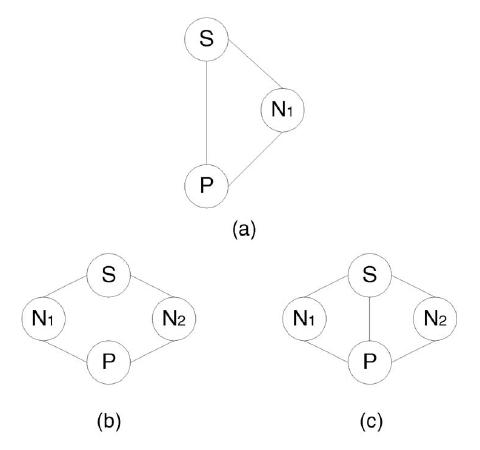
\includegraphics[scale=0.4]{img/ltm_multid.jpeg}
%\caption{Peer $P$ receives $d(i, S, v)$ multiple times}
%\label{figure:ltm_multid}
%\end{figure}
%
%\begin{figure}
%\centering
%  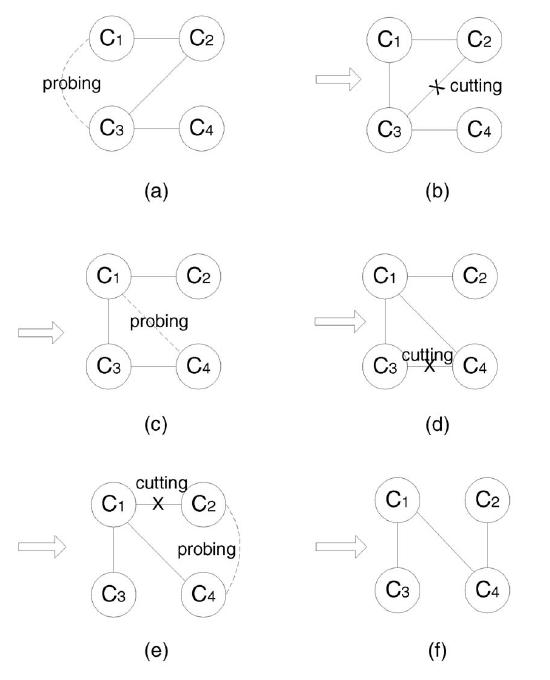
\includegraphics[scale=0.4]{img/ltm_example.jpeg}
%\caption{A full example of LTM}
%\label{figure:ltm_example}
%\end{figure}
%
%\subsection{Scalable Bipartite Overlay}
%\emph{Scalable Bipartite Overlay (SBO)} \cite{liu_bipartite_2007} employs an efficient strategy to select query forwarding paths and logical neighbours. The topology construction and optimization of SBO consist of four phases:
%\begin{enumerate}[\itshape i\upshape)]
%  \item When a new peer is joining the network, it will randomly take an initial colour; say red or white. This colour is not to be changed for the time the peer stays connected. If it leaves and then rejoins it will, again, have to pick a colour, randomly. Thus all peers are separated into two groups, red or white. Then the bootstrap host will provide, the joining peer, with a list of active peers, including their colour information, in order for the later to establish connections to different colour peers. This way, all peers form a bipartite overlay.
%  \item White peers probe distances with their immediate (red) neighbours, form a cost table and send this table to their corresponding red neighbours.
%  \item Each red peer builds a minimum spanning tree using the obtained neighbour cost tables. These are two-hop diameter trees so white peers do not need to build one. The links that are part of a minimum spanning tree are called \emph{forwarding connections (FC)} while the rest \emph{non-forwarding (NFC)}.
%  \item Having a minimum spanning tree with two hops a red peer is able to send its queries within that range. Some white peers, though, have become non-forwarding neighbours. In this phase, such a (white) neighbour will try to find another red peer being two hops away from its current red neighbour to replace the later as its new neighbour.
%\end{enumerate}
%
%\begin{figure}
%\centering
%  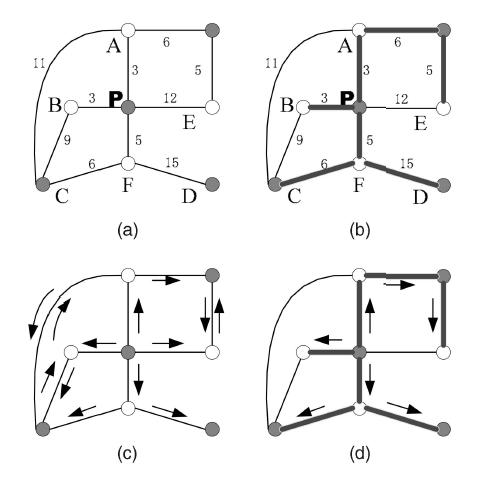
\includegraphics[scale=0.4]{img/sbo_efficient_forward.jpeg}
%\caption{A red peer $P$ has a small overlay topology of $N(P)$ and $N^2(P)$ and computes the efficient forwarding paths}
%\label{figure:sbo_efficient_forward}
%\end{figure}
%
%\begin{figure}
%\centering
%  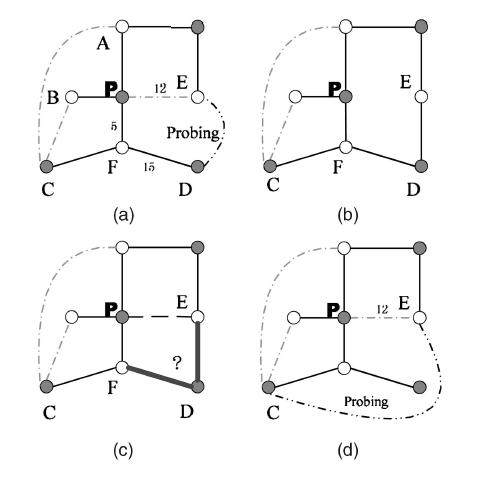
\includegraphics[scale=0.4]{img/sbo_neighbour_replace.jpeg}
%\caption{Neighbor replacement}
%\label{figure:sbo_neighbour_replace}
%\end{figure}
%
%In a static enviromnent LTM may reduce traffic cost by around 80 to 85 percent while SBO reduces traffic cost between 85 and 90 percent. However, LTM  is proved to converge in around 2-3 steps while SBO needs 4-5 steps. Moreover LTM reduces response time by more than 60 percent in 3 steps while SBO needs 8. In a dynamic environment (10 minute average peer lifetime, 0.3 queries/sec by each peer) SBO and LTM reduce the average traffic cost per query (including the overhead due to the optimization steps) by 85 and 80 percent, respectively. Moreover LTM reduces the response time per query to 30 percent while SBO to 35 percent.
%
%\subsection{Adaptive Connection Establishment}
%
%\paragraph{}
%\emph{Adaptive Connection Establishment (ACE)} \cite{liu_ace_2004} builds an overlay multicast tree among each source node and the peers within a certain diameter from the source peer and optimizes the neighbour connections that are not in that tree.
%
%\paragraph{}
%ACE indicates three phases for its algorithm:
%\begin{enumerate}[\itshape i\upshape)]
%  \item Calculate cost between nodes using network delay as a metric. Each peer probes the costs with its immediate logical neighbours and forms a \emph{neighbour cost table (NCT)} using a special routing message type. Two neighbouring peers exchange their NCTs in order for every peer to obtain the cost between any pair of its local neighbours forming a small overlay topology.
%  \item Based on obtained NCTs a minimum spanning tree among each peer and its immediate neighbours is built (Figure~\ref{figure:ace_phase2}).
%  \item Physically far away neighbours are replaced by physically close neighbours. In ACE a peer, say $S$, probes the distance between one of its non-flooding neighbour's neighbour, say $G$ and $H$ respectively. If the link to neighbour's neighbour is smaller than that to the neighbour, the later is cut. If this is not the case but $S$ finds that cost of $GH$ is even larger than that of the $SH$, $S$ will keep $H$ as a new neighbour. Obviously, if $SH$ is larger than $SG$ and $GH$, the connection will not be established and $S$ will continue probing another neighbour's neighbour. The algorithm described is conducted within $1$-neighbour closure (among its source peer and all its direct neighbours) but the optimization scope can be enlarged. The larger the scope, the better topology matching improvement but also the greater the computational overhead (Figure~\ref{figure:ace_phase3}).
%\end{enumerate}
%
%\paragraph{}
%Simulations in \cite{liu_acesims_2004} show that the average scope of each query to cover the same scope of nodes is reduced by about 65 percent without losing any autonomy feature, while the average response time can be reduced by 35 percent. Larger diameter topologies lead to better topology optimization rate but also to higher communication and computation overhead. It was also found that it is more effective in higher connectivity dense topologies. Compared to LTM, it comes short of convergence speed. In \cite{ni_mismatch_2004} shows reduction of both total traffic (90 percent) and response time (80 percent) to message queries without shrinking the search scope. SBO, on the other hand, achieves approximately 85 percent reduction on traffic cost and about 60 percent reduction on query response time. Last but not least, it is concluded that work must be done on incorporating a more sophisticated selection policy for candidate non-flooding peers.
%
%\begin{figure}
%\centering
%  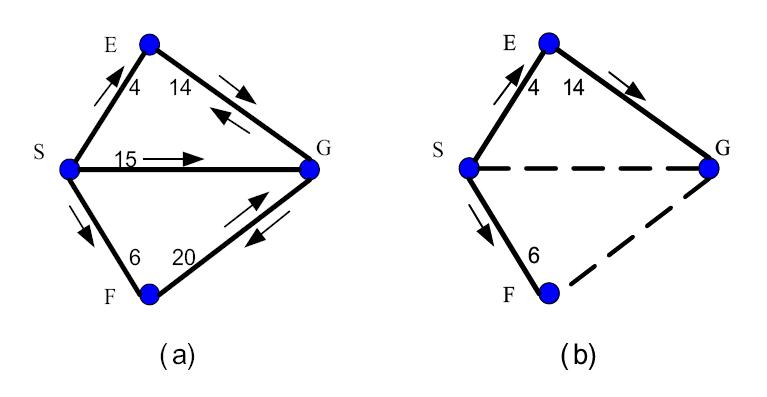
\includegraphics[scale=0.4]{img/ace_phase2.jpeg}
%\caption{Second phase in ACE}
%\label{figure:ace_phase2}
%\end{figure}
%
%\begin{figure}
%\centering
%  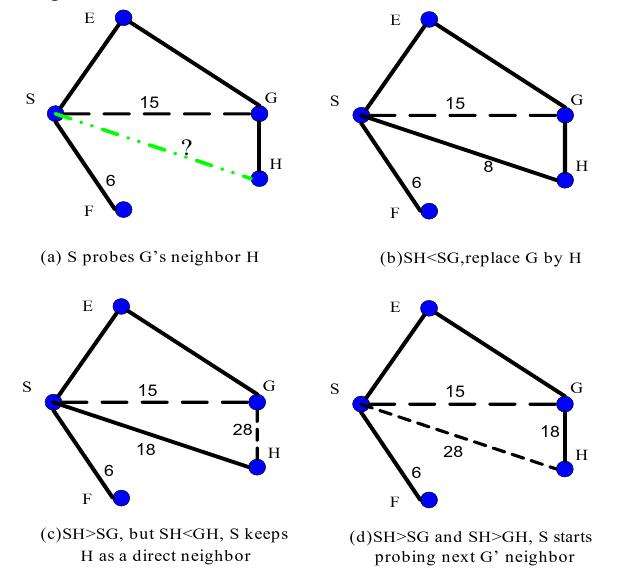
\includegraphics[scale=0.4]{img/ace_phase3.jpeg}
%\caption{Third phase in ACE}
%\label{figure:ace_phase3}
%\end{figure}
%
%\subsection{Hops Adaptive Neighbour Discovery}
%
%\paragraph{}
%Paper \cite{chen_hand_2006} proposes a new algorithm named \emph{Hops Adaptive Neighbour Discovery (HAND)} which uses a fully distributed triple hop adjustment strategy to address the topology mismatch problem. The advantages of the algorithm compared to other approaches are that
%\begin{inparaenum}[\itshape i\upshape)]
%  \item it does not need any clock synchronization,
%  \item it is a fully distributed algorithm making it robust and reliable in decentralized systems,
%  \item the traffic overhead of the triple hop adjustment is very low,
%  \item it is applicable to dynamic peer-to-peer environments, and
%  \item maintains lower query response time.
%\end{inparaenum}
%
%\paragraph{}
%The algorithm's ultimate goal is the optimal overlay, the \emph{Logical Communication Network (LCN)} in the paper's context. The key concept of the algorithm is that a graph $G^{*}$ that describes an LCN and a graph $G$ that describes the current overlay are matched only if all peer hop sequences $(v_1, v_2, \ldots, v_k)$ in $G$ exist in $G^{*}$ and in the same order. In practice triple sequences $(v_1, v_2, v_3)$ are used.
%
%\paragraph{}
%The mismatching detection is done in the following way. Suppose we want to verify peer sequence $v_2-v_1-v_3$ (see Figure~\ref{figure:hand_com_overlay}). A pair of probing messages are sent from $v_1$ to $v_2$ and $v_3$. Suppose delays of $(v_1,v_2)$ and $(v_1,v_3)$ are are denoted as $x$ and $z$, respectively. When the probing message arrives to $v_2$ it forwards it directly to $v_3$. Similarly, when the probing message arrives to $v_3$, it forwards it directly to $v_2$. These last steps are performed in order to obtain delays of $(v_2,v_3)$ and $(v_3,v_2)$ physical paths, respectively, denoted by $y$.
%\begin{itemize}
%  \item If $y=z-x\pm\varepsilon$, sequence $v_2-v_1-v_3$ is mismatched and should be adjusted to $v_1-v_2-v_3$ by deleting edge $(v_1,v_3)$ and adding a new $(v_2,v_3)$ (see Figure~\ref{figure:hand_matchtriple_lemma3}).
%  \item if $y=x-z\pm\varepsilon$, sequence $v_2-v_1-v_3$ is mismatched and should be adjusted to $v_1-v_3-v_2$ by deleting edge $(v_1,v_2)$ and adding a new $(v_3,v_2)$ (see Figure~\ref{figure:hand_matchtriple_lemma4}).
%\end{itemize}
%$\varepsilon$ is a small positive real number denoting additional delays caused by possible forwarding and jitter delays.
%
%\begin{figure}
%\centering
%  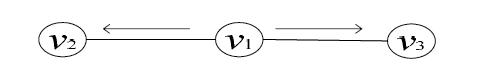
\includegraphics[scale=0.4]{img/hand_com_overlay.jpeg}
%\caption{The communication in overlay}
%\label{figure:hand_com_overlay}
%\end{figure}
%
%\begin{figure}
%\centering
%  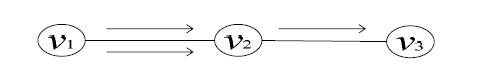
\includegraphics[scale=0.4]{img/hand_matchtriple_lemma3.jpeg}
%\caption{The matching triple in paper's Lemma 3}
%\label{figure:hand_matchtriple_lemma3}
%\end{figure}
%
%\begin{figure}
%\centering
%  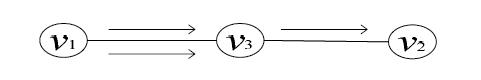
\includegraphics[scale=0.4]{img/hand_matchtriple_lemma4.jpeg}
%\caption{The matching triple in paper's Lemma 4}
%\label{figure:hand_matchtriple_lemma4}
%\end{figure}
%
%\paragraph{}
%Measurements conducted for evaluation perposes showed that in a static environment the algorithm can effectively decrease traffic cost by about 77 percent and shorten the query response time by about 49 percent in less than two minutes. In a dynamic environment it shows similar behaviour and with the size of the overlay network having little impact on the effectiveness of the algorithm. Compared to LTM both algorithms have almost the same traffic reduction rate, however on the response time reduction rate HAND has a higher one by about 4 percent. The traffic overhead of HAND is much less than that of LTM by an average of 55 percent.
%
%\subsection{Distributed Cycle Minimization Protocol}
%
%\paragraph{}
%\emph{Distributed Cycle Minimization Protocol (DCMP)} which is introduced in \cite{zhu_dcmp_2008} is a dynamic, fully decentralized protocol that promises significant reduction of duplicate messages. To achieve that, it uses the slightly different approach of eliminating unnecessary cycles, while retaining the connectivity of the network and preserving fault resilience and load balancing properties of unstructured peer-to-peer schemas by avoiding the creation of a hierarchical organization.
%
%DCMP aims at cutting the cycle paths at strategic locations. Any peer that detects a duplicate message can initiate the cutting process which consists of the following steps:
%\begin{enumerate}
%  \item Peers in the cycle elect a leader called \emph{GatePeer}\footnote{GatePeers are important for maintaining the connectivity and optimal structure of the network while peers join and leave randomly.}.
%  \item The cycle is cut at a well-defind point with respect to the GatePeer
%\end{enumerate}
%
%\paragraph{}
%The first step after detecting a duplicate message by some peer is to gather information from all peers in the cycle using a new type of control message called \emph{Information Collecting Message} or \emph{ICM}. ICM contains:
%\begin{inparaenum}[\itshape i\upshape)]
%  \item a \emph{GUID}\footnote{Globally Unique IDentifier assigned to every query message generated by any node.} field same as the one of the duplicate message,
%  \item \emph{DetectionID} field which represents the direction of the connection where the duplicate was identified\footnote{This ensures the uniqueness of the ICM messages because as it travels through many cyclic paths, multiple peers will detect the duplicates and initiate an ICM message.}, and
%  \item \emph{Node Information Vector (NIV)} which contains information (bandwidth, CPU power, etc) about peers that propagated the ICM.
%\end{inparaenum}
%
%\paragraph{}
%Suppose $A$ detected the duplicate as depicted in Figure~\ref{figure:dcmp}. It then emits an ICM to $B$ and $F$, that initially contains information only about itself. Each peer that receives the ICM, appends its information and propagates it along the reverse path of the original message. Since two copies of ICM are sent, at some point, a peer, say peer $D$, will receive a duplicate ICM. Using the information in the NIVs of the ICMs, $D$, decides to cut (for example) the EF connection. To inform the other peers about its decision, it emits a \emph{Cut Message (CM)} which contains the GUID and DetectionID of the corresponding ICM and an additional field that identifies the connection to be cut. $D$, then, forwards the CM in the reverse directions from where the ICM arrived. Similarly CMs received by any peer are propagated toward the reverse path of the corresponding ICM. Eventually, either peer $E$ or peer $F$ will receive the CM and cut the connection, thus eliminating the cycle.
%
%Receiving a duplicate ICM denotes the existence of a cycle. The opposite is not true though. For example, if the cycle contains $2 \times TTL$ edges, it will not be detected, because the ICM messages will be discarded before they locate it. There is a tradeoff between preserving the connectivity of the network and minimizing the duplicates that makes such a possibility to be safely ignored.
%
%\begin{figure}
%\centering
%  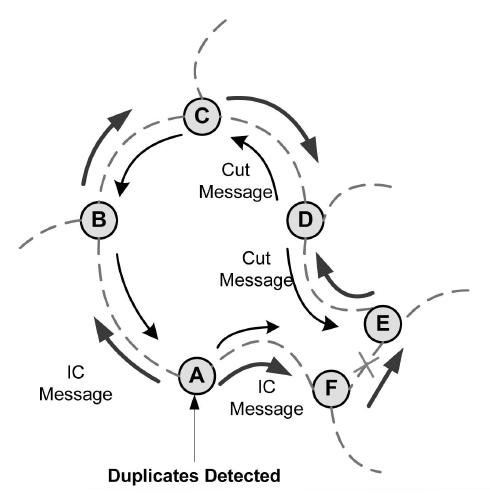
\includegraphics[scale=0.4]{img/dcmp.jpeg}
%\caption{Cycle elimination methods in DCMP}
%\label{figure:dcmp}
%\end{figure}
%
%\paragraph{}
%Experiments in \cite{zhu_dcmp_2008} showed that DCMP incurs a lower delay, returns more results and decreases the number of duplicate messages by 22\%, compared to LTM. Additionally DCMP has one to two orders of magnitude less overhead, because it adopts a more ``LAZY'' approach than broadcasting control messages periodically like LTM does.
%
%\subsection{Two-Hop-Away Neighbour Comparison and Selection}
%
%\paragraph{}
%Work in \cite{liu_thancs_2005,liu_thancs_2008} proposes a distributed heuristic called \emph{Two-Hop-Away Neighbour Comparison and Selection (THANCS)} that
%\begin{inparaenum}[\itshape i\upshape)]
%  \item is completely distributed and needs no global knowledge,
%  \item presents trivial overhead compared to the query cost savings
%  \item its convergent speed of the algorithm is fast enough (faster than minimum spanning tree approaches) so that is effective to dynamic environments, and
%  \item does not shrink the search scope.
%\end{inparaenum}
%
%\paragraph{}
%THANCS is considered a \emph{local search method}, in the sense that it targets in finding a locally optimum solution, by exploiting knowledge within a 2-hop radius. The algorithm consists of two main components: \emph{piggybacking neighbour distance on queries} and \emph{neighbour comparison and selection} which are furtherly discussed bellow.
%
%\paragraph{Piggybacking neighbour distance on queries}
%Using network delay as a metric for measuring the distance, each peer probes distances with its immediate naighbours and stores information locally. For this reason a special query message type, \emph{Piggy Message (PM)}, is introduced. It is 6 bytes long and includes two fields: Neighbour IP Address and Neighbour Distance. A peer $P$ constructs a PM for its neighbour $Q$, which contains $Q$'s IP address and $Q$'s distance from $P$. When $P$ receives a query from $Q$, this PM will be piggybacked by the query that goes to all other neighbours of peer $P$. Upon receiving such a query message, each of the other neighbours will detach the PM, record the $PQ$ distance and process the query. This PM will not be further forwarded. In selecting which incoming queries  should piggyback a PM the paper proposes the \emph{pure propability-based (PPB)} and the \emph{new neighbour triggered (NNT)} policies.
%
%\paragraph{Neighbour comparison and selection}
%Figure~\ref{figure:thancs} illustrates this component of the THANCS algorithm. A peer $S$ probes the distance to all known unprobed $N^2(S)$\footnote{$N^2(S)$ denotes the set of peers being two hops away from $S$, while $N(S)$ denotes the set of direct logical neighbours of $S$.}. The distance of $SP$ is known to $S$. Upon receiving a PM from node $P$ with the distance of $PQ$, $S$ follows one of the following:
%\begin{itemize}
%  \item $Q \in \left( N(S) \cap N^2(S) \right)$, i.e. $Q$ is direct neighbour of $S$. In this case $S$ will compare cost of $SQ$, $SP$ and $PQ$. If the most costly connection is one of $SQ$ or $SP$ the corresponding link will be put into a \emph{will-cut list}\footnote{Links are not immediately disconnected when put in the will-cut list. There are useless for forwarding but are kept active, for some time, in order to serve query responses that are traveling to the source peer along the inverse search path.}. If the most costly connection is $PQ$ then $S$ will do nothing, as the fully distributed nature of the algorithm will give a chance to either $P$ or $Q$ to cut the connection.
%  \item $Q \in \left( N^2(S) - N(S) \right)$, i.e. $Q$ is a two-hop-away neighbour of $S$. If $S$ hasn't probed $Q$ before\footnote{A distance cache is maintained and looked up in such a case.}, it probes and stores the result in the \emph{distance cache}. Having the distance of $SQ$, $S$ compares costs of $SQ$, $SP$ and $PQ$. If $SQ$ is the most costly, $S$ will not establish the connection. If $SP$ is the most costly, $S$ will establish connection $SQ$ and put $SP$ in the will-cut list. If $PQ$ is the longest, $S$ will keep  the connection with both $P$ and $Q$, expecting that $P$ or $Q$ will eventually disconnect link $PQ$, later.
%\end{itemize}
%
%\begin{figure}
%\centering
%  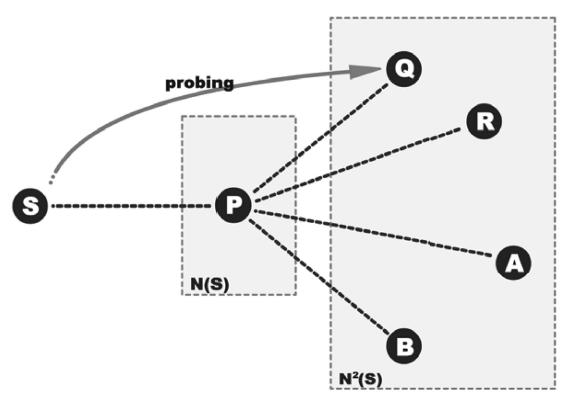
\includegraphics[scale=0.4]{img/thancs.jpeg}
%\caption{Probing two-hop-away neighbours}
%\label{figure:thancs}
%\end{figure}
%
%\paragraph{}
%In a static environment THANCS has been proven to be effective; optimizing 45 percent out of the 60 percent of mismatched paths, constructing a nearly optimal overlay. This leads to a 60 percent reduction in traffic cost as well as a 40 percent decrease in query response time. In dynamic environments (Gnutella 0.6/Limewire super-peer-like and Ion flat-like), THANCS saves up to 70 percent of the traffic cost in the super-peer topology and 55 percent for the flat one. Average response time is also decreased by 60 and 45 percent, respectively. Generally, THANCS has similar performance to LTM, without needing synchronization. SBO, incurring half the  overhead of AOTO, reduces the traffic cost the most, while THANCS has lower response time and converges faster than SBO. THANCS is, thus, more suitable for a more dynamic environment. In addition, THANCS is easy to implement and its operation overhead is trivial, compared with the other three approaches. This design, however, has the limitation of not being easily extend to also support non-flooding-based systems.
%
%\subsection{mOverlay}
%Zhang et al. in \cite{zhang_moverlay_2004} focus on two aspects of the overlay construction. First, to achieve \emph{efficiency} of communication, a protocol should minimize unecessary long-distance hops and redundant traffic. Second, to be \emph{scalable} the overlay should be constructed in a distributed fashion and maintenance cost (data and locality management) should be minimized. Both of the above observations, are positively affected by the exploitation of node proximity at the underlying network. To accomplish it, the paper introduces the \emph{group} concept, according to which non-static (dynamic) landmarks are used to compute proximity, resulting in a highly robust and scalable overlay construction with reduced maintenance cost as well. The dynamic nature of landmarks help towards load-balance, meaning that hot-spots are avoided.
%
%\paragraph{}
%The proposed architecture, called \emph{mOverlay}, is a \emph{clustering approach} which creates a two-level hierarchical network, where on the top level we have connections between groups while on the bottom we have connections between hosts inside groups, thus attempting to recreate \emph{Small-World}-like properties for the constructed overlay network. The notion of a \emph{group}, in the paper's context, is a set of hosts that are close to each other with respect to any position $P$ in the underlying network. The distance between hosts can be 
%\begin{inparaenum}[\itshape i\upshape)]
%  \item network latency,
%  \item round-trip time,
%  \item minimum bandwidth on the links along the path connecting the two nodes, or
%  \item some other user-defined cost metric between the two nodes.
%\end{inparaenum}
%These nodes are refered to as neighbouring. Similarly groups can exchange messages with their neighbouring ones\footnote{Groups nearby, in the underlying physical network.}.
%
%According to the \emph{grouping criterion} set by the authors, a new host $Q$ belongs to some group $A$ if the distance between $Q$ and group $A$'s neighboring groups is the same as the distance between group $A$ and it's neighbouring groups. The neighbour groups thus, play the role of the dynamic landmarks and for accuracy and performance reasons the nearest of them are chosen to play that role.
%
%\paragraph{Locating process} A new coming host, $Q$, first connects to a globally known host cache called the \emph{rendezvous point (RP)} in order to retrieve the starting point in the overlay, say $A$ in group $1$. Host $Q$ then, measures its distance to host $A$. At the same time, the later, sends information about the neighbour groups of group $1$ back to host $Q$. This list is called \emph{candidate group list}, and the newcoming host sequnentially measures its distance to each of them in seek for the closest one. If the \emph{grouping criterion} is met, host $Q$ belongs to group $1$. If not, a boot host from the closest group is found and the algorithm is re-run until the criterion is met or after a predefined number of repetitions. In the later case, $Q$ creates a new group comprising itself only. The above protocol does not favour hotspots as it spreads the probability of visiting a group across the whole overlay and limits the overhead in the level of $O \left ( log N \right )$.
%
%\paragraph{General overlay operations} A set of additional protocols, are also introduced, similar to those found in traditional unstructred networks, but modified focusing on scalability and robustness. For example a protocol for \emph{group formation} is introduced that exploits the inherent characteristic of proximity, in the overlay, in order to efficiently detect the neighbouring groups of a newly formated group from the set of adjasent groups of its closest neighbour. Additionaly, during \emph{group joining} the coresponding protocol denotes the exchange of important information for group maintenance. This can be furtherly improved by \emph{information sharing} between nodes of the same group, functionality handled by a dedicated flood-like protocol\footnote{Since nodes that belong to the same group are physically close this can be achieved at a minimum price.}. Moreover, another set of distributed protocols handle the \emph{information update}. The information that needs update, in the proposed architecture, is
%\begin{inparaenum}[\itshape i\upshape)]
%  \item the host cache, when a new node joins, and
%  \item the neighbours of groups, when a close-by group is generated.
%\end{inparaenum}
%Finally, in case of \emph{host failure} or \emph{host departure} the system is able to maintain its stability since there are defined operations for periodical host cache update and group leader selection if one leaves or dies.
%
%\subsection{Distributed Domain Name Order}
%{\sethlcolor{yellow}\hl{HA:  In paper/introduction nice advantages of unstructured networks:
%
%Unstructured P2P networks o?er a number of
%important advantages: (i) An unstructured network
%imposes very small demands on individual nodes,
%and more speci?cally it allows nodes to join or leave
%the network without signi?cantly a?ecting the sys-
%tem performance. (ii) Unstructured networks are
%appropriate for content-based retrieval (e.g., key-
%word searches) as opposed to object identi?er loca-
%tion of structured overlays. (iii) Finally unstructured
%networks can easily accommodate nodes of vary-
%ing power. Consequently, they scale to very large
%sizes and they o?er more robust performance in
%the presence of node failures and connection
%unreliability.
%}}
%
%\paragraph{}
%\cite{zeinalipour-yazti_ddno_2005} proposes the \emph{Distributed Domain Name Order (DDNO)} technique which makes unstructured overlay networks, topologically aware. It results in a flat overlay topology but with some changes it can be utilized in \emph{superpeer} environments. In DDNO, a node of degree $d$, tries to connect to $\frac{d}{2}$ nodes that belong to the same domain (\emph{sibling} connections) and another $\frac{d}{2}$ of random nodes (\emph{random} connections). Connecting to \emph{sibling} nodes ensures the reduction of long distance message travelling and thus resulting to better performance, while \emph{random} nodes keep the structure connected.
%
%\paragraph{Discovering \emph{random} neighbours}
%Initially, when a new coming node wants to join a network $N$, uses a \emph{hostcache} mechanism to provide it with a list of nodes with which to establish its $\frac{d}{2}$ \emph{random} connections.
%
%\paragraph{Discovering \emph{sibling} neighbours}
%In order to discover the rest $\frac{d}{2}$, \emph{sibling}, nodes, the \emph{lookupDN} procedure is initiated. In this phase, a special $l$ walker message is multicasted, by the newcomer, in search of a node that knows\footnote{A special structure is used called ZoneCache that contains information about which nodes are reachable in an $r$-hop radius.} how to guide $n$ to a \emph{sibling} node.
%
%\paragraph{}
%Figure~\ref{figure:ddno_lookupdn} shows an $l$ message emitted by node $n$ which travels along the path [$a$, $b$, $c$, $e$, $b$, $d$]. At node $d$, $l$ finds information to make a decision on which neighbour to follow next\footnote{Contrary to the random choices, made at the previous hops.}. Ultimately $l$ arrives at $m$, which is a \emph{sibling} node to $n$. $m$ then issues a broadcast message to all its own \emph{siblings}. Each of the receiving nodes, $m$ included, will respond to $n$ with a designated $l^{'}$ message if it is willing to accept new connections and out of these answers, node $n$, will attempt to establish its, remaining, $\frac{d}{2}$ \emph{sibling} connections.
%
%\paragraph{}
%Unfortunately, use of DDNO results in networks which have a uniform distribution of node degrees, losing the valuable properties of Power Law and Small World networks, as mentioned previously in this survey.
%
%\begin{figure}
%\centering
%  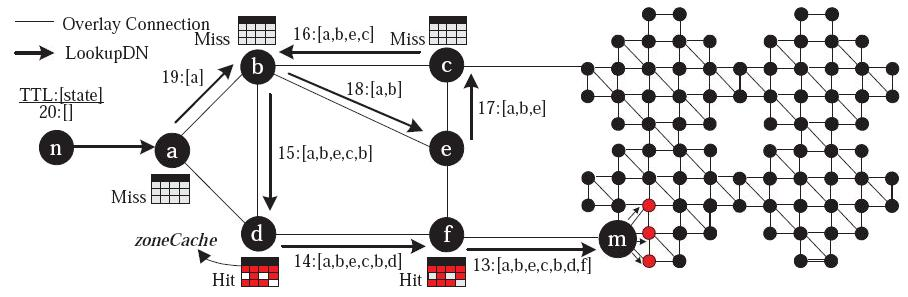
\includegraphics[scale=0.375]{img/ddno_lookupdn.jpeg}
%\caption{Domain name look-up in a \emph{DDNO} topology}
%\label{figure:ddno_lookupdn}
%\end{figure}
%
%%\subsection{Critical Topology-Aware Grouping}
%%
%%\paragraph{}
%%\emph{Critical Topology-Aware Grouping (CTAG)} presented in \cite{zhao_ctag_2006}, is a grouping algorithm that tries to exploit low-cost and low-delay communication of physically close-by peers. The grouping strategy is based on the \emph{IANA}\footnote{Internet Assigned Numbers Authority} and the respective \emph{Regionanal Internet Registry (RIR)}'s IP assignment strategies, according to which nodes within the same organization are always addressed from the same block. The paper proposes the \emph{Adjacency Measurement (AM)} technique which uses the longest matching IP segment criterion to calculate node proximity.
%%
%%Observations made in various studies (e.g. \cite{matei_mapgnutella_2002}) concerning the distribution of nodes among \emph{Internet Service Providers (ISPs)} and \emph{Autonomous Systems (ASs)} have shown that only $2$ to $5$ percent of Gnutella connections link peers within a single AS while more than $40$ percent of all Gnutella peers are located within the top 10 ASs. Similarly, measurements in \cite{zeinalipour-yazti_gnudc_2002} used a $244,000$ IPs test-bed and results have shown that $45$ percent of the nodes belonged to only $10$ large ISPs and $58$ percent belong to only $20$. Such results mean that most overlay generated traffic crosses AS borders increasing topology mismatch cost.
%%
%%\emph{CTAG} focuses on both the construction of the overlay as well as dynamically revising it during node interaction, phases called \emph{bootstrapping grouping} and \emph{dynamic revision}, respectively in the paper's context.
%%
%%\paragraph{Bootstrapping grouping}
%%The \emph{Gnutella Web Caching} mechanism has been modified in order for a new coming node to choose the closest \emph{GWC} in order to retrieve the node list for bootstrapping.
%%
%%\paragraph{Dynamic revision}
%%Similarly to the bootstrapping phase, \emph{AM} metric is used to store hosts' addresses. read from \emph{X-Try} headers during handshake or from \emph{QueryHit} messages. Additionally, when a node reaches the max neighbour connections, node disconnects the neighbours with the lowest \emph{AM}.
%
%\subsection{Peer-exchange Routing Optimization Protocols}
%
%\paragraph{}
%Work presented in \cite{qiu_prop_2007} introduces \emph{peer-exchange}\footnote{A series of exchanges of neighbours between two peers. One exchange can be viewed as a pair of cut-add operations.} as a basic operation to adaptively adjust the connections of the overlay network, and efficiently reduce the average logical link latency of the whole system. There are two points that differentiate this scheme from others:
%\begin{inparaenum}[\itshape i\upshape)]
%  \item it utilizes the collaboration of two peers to optimize their neighbourhood environment, than simply letting each node to ``selfishly'' choose its own strategy, and
%  \item can be deployed effortlessly on both unstructured and structured peer-to-peer systems.
%\end{inparaenum}
%
%\emph{PROP-G}\footnote{\emph{G} stands for \emph{generic}.} is the simple and direct variant of \emph{peer-exchange} in which two neighbours swap all their neighbours. As depicted in figure~\ref{figure:prop-g} the mechanism can be viewed as, nodes, exchanging overlay ``positions''. Thus, the overall overlay topology is not affected by the this operation.
%
%\begin{figure}
%\centering
%  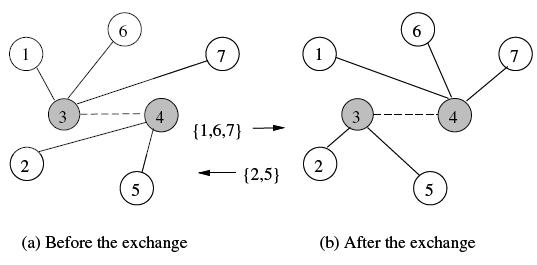
\includegraphics[scale=0.4]{img/prop-g.jpeg}
%\caption{PROP-G in which a neighbours are exchanged.}
%\label{figure:prop-g}
%\end{figure}
%
%The alternative protocol proposed, called \emph{PROP-O}\footnote{\emph{O} stands for optimized}, ensures that the degree of each participating node remains the same by selectively choose the same number of neighbours for the exchange. With this mechanism, 2 nodes exchange the same number of neighbours in order not to change the degree
%
%\begin{figure}
%\centering
%  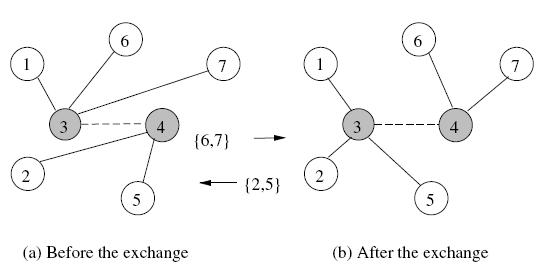
\includegraphics[scale=0.4]{img/prop-o.jpeg}
%\caption{PROP-O exchanging \emph{m} neighbours.}
%\label{figure:prop-o}
%\end{figure}
%
%\subsection{T2MC}
%
%\paragraph{}
%\emph{T2MC}\cite{shi_t2mc_2008} exploits some properties of the Internet paradigm and clusters nodes belonging to the same ISP without any centralised control or predefined system parameterization. The algorithm considers the dynamic nature of peers and exploits the stable nature of routers in order to build a topology location relationship among end peers.
%
%\paragraph{}
%Some special routers split the physical network into autonomous system domains. Using a Traceroute mechanism T2MC searches for latency leaps among the path to a host in order to form ``near'' and ``remote'' router clusters. This is achieved by a 2-Means Classification, defined by the following steps:
%\begin{enumerate}
% \item the peer chooses the minimum and maximum Latency results from the Traceroute for initializing the cntroinds of two sets ``first'' and ``second''.
% \item The peer calculates, for all hops allong its tracerouted path, the absolute distance to the centroids of both sets and assigns the routers to that centroid with which it has the smaller absolute distance.
% \item The peer calculates the latncy mean and variance value of two sets
% \item If the variance is larger than a predefined threshold then the algorithm takes a loop from step 2 picking the two latency mean values as new centroids of sets ``first'' and ``second''.
%\end{enumerate}
%Ultimately peer will end up with two sets having the minimum intra-set variance. Finally the peer chooses the router from ``second'' set with the minimum hops attribute and sets it as a threshold. The selected router and all others whose hops attribute is larger than the threshold are classified as ``remote'' router cluster. The remaining are classified as ``near''. From the ``near'' class, the peer chooses the one with maximum hops attribute as its edge router, and registers it along with the all the ``near'' cluster into the DHT of the p2p overlay. As new peers join the network, those that share the same edge router or any of the members of the ``near'' router clustersm ther would gather to form a ``close'' peer cluster. As Edge routers can provide more valuable information than other members of the ``near'' set, T2MC was designed to prioritize interaction of peers and edge gateways.
%
%% TODO: figure t2mc.jpeg (a) stars represent edge routers (b) hop leaps
%
%\paragraph{}
%The use of Traceroute as a tool for implementing the distance measuring infrastructure raise concearns about its efficiency and scalability. Being, primarilly, a network diagnostic utility, it is concearned too heavy weighted and intrucive for use in a larger scale\cite{ratnasamy_binning_2002}. Additionally, disabling ICMP is a common administrative policy for edge sites to enforce security, while dumping BGP routing tables\cite{krishnamurthy_bgpclust_2000} is not directly available to the application layer.
%
%\subsection{Unnamed Unstructured!!}
%% TODO: to be reviewed
%
%\paragraph{}
%In \cite{hsiao_redblue_2009}, Hsiao et al, claim to construct topology-aware unstructured overlays that \emph{guarantee} performance qualities in terms of
%\begin{inparaenum}[\itshape i\upshape)]
%  \item the expected communication latency among any two overlay peers regardless of the network size, and
%  \item the broadcasting scope of each participating peer.
%\end{inparaenum}
%
%The algorithm constructs an undirected graph $G = \left( V, E \right)$ comprised by two subgraphs. The first, namely $G^{\left( red \right)} = \left( V^{\left( red \right)}, E^{\left( red \right)} \right)$ in the paper's context, includes all vertices of $G$ and ensures the connectivity of the graph by securing at least one path between any two nodes. In contrast, $G^{\left( blue \right)} = \left( V^{\left( blue \right)}, E^{\left( blue \right)} \right)$, contains those vertices of $G$ that have free edges to link to other nodes and because these are fully utilized, the following also stands $E = E^{\left( red \right)} \cup E^{\left( blue \right)}$.
%
%A joining peer $u$, partitions its neighbours into two subsets, the $B_u^{\left( red \right)}$ and $B_u^{\left( blue \right)}$. In order to populate the $B_u^{\left( red \right)}$ subset, peer $u$ samples peers uniformly and at random. Then, each of these selected peers discovers a routing path starting from itself towards the node with the smallest (or the largest) ID in the system.
%
%%%%%%%%%%%%%%%%%%%%%%%%%%%%%%%%%%%%%%%%%%%%%%%%%%%%%%%%%%%%%%%%%%%%%%%%%%%%%%%%
%% STRUCTURED
%%%%%%%%%%%%%%%%%%%%%%%%%%%%%%%%%%%%%%%%%%%%%%%%%%%%%%%%%%%%%%%%%%%%%%%%%%%%%%%%
%
%\subsection{Landmark Binning}
%The scheme proposed in \cite{ratnasamy_binning_2002} is based on the process of \emph{binning} close by nodes (in terms of network latency) into the same cluster. The authors set the following objectives for designing their proposed algorithm:
%\begin{enumerate}
% \item simplicity (minimal support from any measuring infrastructure),
% \item scalablility (no global knowledge of the network),
% \item complete distribution (nodes need no communication-cooperation).
%\end{enumerate}
%
%\paragraph{Binning scheme}
%The implementation requires a set of well-known \emph{landmark} machines spread accross the Internet. Every newly arriving node measures its distance from these landmarks and unilaterally decides to join a specific bin based on these results. In more detail the node measures its round-trip time to each of the landmarks and orders these measurements in a decreasing order. The ordering represents a ``bin'', in the sence of close-by nodes having the same landmark ordering and hance belong to the same ``bin''. This means that a landmark system consisting of $m$ such nodes results in $m!$ potentional different bins.
%
%The algorithm can be considered scalable, as nodes need only compute distances to a small number of predefined nodes and thus without exchanging any information. A potential bottleneck could be the extra load that this ``ping''-like scheme imposes to the landmarks, especially when we need instant reaction from our topology when dealing with the dynamic nature of the p2p networks.
%
%To answer the question as to whether the algorithm actually contributes possitivelly to the construction of an enhaned overlay, the paper defines the \emph{gain ratio} as the factor by which the latency reduces when someone communicates with a random node from the same bin than with one not in the bin. This is implemented with an inter-bin to an intra-bin latency ratio.
%
%\paragraph{Structured and Unstructured Binning}
%The \emph{binning} scheme can be incorporated within either a structured or an unstructured overlay construction algorithm. The authors provide an example for both these cases.
%
%\paragraph{}
%Assuming a structured approach based on CAN\cite{ratnasamy_can_2001} and $m$ landmark nodes. The coordinate space is then partitioned into $m!$ equally sized portions, each corresonding to a single ordering of the landmarks. To do this, the first dimension is divided into $m$ areas each of which is furtherly divided (second dimension) into $m - 1$ sections and so on. Having set this $m$ dimensional space, at joining time, a node measures the delay to the set of landmarks in order to determine its associated bin and thus position itself in that portion of the coordinate space associated with its landmark ordering. Even though this scheme can 
%
%For unstructured overlays the paper assumes \emph{a set of $n$ nodes where each node picks any $k$ neighbour nodes so that the average routing latency on the resultant overlay is low (assuming shortest path routing)}. According to the proposed heuristic algorithm called \emph{BinShort-Long}, a node picks its neighbours by choosing its $\frac{k}{2}$ closest\footnote{If the node's bin is not large enough for it to pick these $\frac{k}{2}$ neighbours, it picks the required nodes from the bin that matches the most in terms of landmark ordering.} ones (named \emph{short links}), using the \emph{binning} scheme and the rest $\frac{k}{2}$ randomly (\emph{long links}). The former set produces well-connected \emph{pockets} of nearby nodes while the later preserves the connectivity of the graph, both yielding a proximity factor of $\alpha = 0.5$ in an attempt to preserve the benefitial properties of unstructured topologies\cite{merugu_str2unstr_2003}.
%
%\paragraph{}
%% TODO double check validity
%One disadvantage of this landmark scheme is related to the additional burden imposed to the landmark sites. The authors claim though that the algorithm requires so little work by the landmarks (maybe just echo to ping messages) that could in effect, act as ``unsuspecting participants''. Even if this is the case, the fact that it is not fully distributed, renders the protocol's scalability directly volnerable to any system size increase as well as usuitable for highly dynamic networks such as ad-hoc networks. Moreover, fixed points in a network are inherently more exposed to malicius attacks. The most significant downside of the algorithm though is that it can lead to an extremely uneven overlay ID distribution causing load inbalances and hot spots. Lastly, the scheme is coarse grained when it comes to distinguishing relatively close nodes\footnote{In the worst case, all nodes could ve clustered into a single bin.}.
%
%\subsection{Global Soft-State}
%{\sethlcolor{yellow}\hl{HA: in paper introduction, discussion about
%disadvantages of top-aware CAN:
%
%Techniques to exploit topology information in overlay
%routing include geographic layout, proximity routing and
%proximity neighbor selection [3]. With geographic layout
%such as topology-aware CAN [12], the overlay structure is
%constrained by underlying network topology. This tech-
%nique, unfortunately, can create uneven distribution of
%nodes in the overlay, increasing the chances of overloading
%nodes and rendering the maintenance cost formidable. Our
%study shows that, for a typical 10,000-node topology-aware
%CAN, 5% nodes occupy 85-98% of the entire Cartesian
%space, and some nodes have to maintain 450-1500 neigh-
%bors. In Proximity routing, physical topology is not consid-
%ered when constructing the overlay.
%
%[snip]
%Studies [14] have shown that triangle inequal-
%ity may not hold in Internet topology. In fact, study from
%Pastry has shown that the proximity approximation is much
%worse when using the Mercator topology that is based on
%the real measurements of the Internet [3].
%
%RELATED WORK:
%
%Miguel Castro et al [3] divide techniques used to
%exploit network proximity into three categories: geographic
%layout, proximity routing and proximity neighbor selection.
%Proximity neighbor selection is superior in terms of load
%balancing and proximity approximation. The existing algo-
%
%}}
%
%\paragraph{}
%The approach argued by Xu et.al in \cite{xu_globstate_2003} is to build a global map to help choose shorter routing paths, combining the landmark binning method and small scale distance probes to reveal the proximity properties of the underlying network to the overlay. This global view of the state is made available to all nodes in order to help them find the best way to route their messages. The authors focus on two aspects in order to accomplish their goal.
%
%\paragraph{}
%Initially, is the \emph{generation} of proximity information and then its \emph{effective exploitation}. For the first, a hybrid approach is proposed, which uses landmark clustering as a preprossesing step in order to select a number of potential nearest neighbour candidates and then refine the selection by incorporating an RTT scheme to ultimately choose the closest node. For the second, the algorithm chooses a different path from the classic gossiping approaches for constructing and maintaining the overlay. It is based on landmark-clustering-based strategic placement of proximity information on the overlay enabling any node to access such information using a landmark number that reflects its physical position in the network. For various logical regions\footnote{This might be a high-order zone in the eCAN\cite{xu_ecan_2002} context or a set of nodes sharing a particular prefix in overlays such as Pastry.} maps of physical information are built and published where each node may appear in a maximum of $log\left( N \right)$ such maps.. To dynamicaly adapt to changing network conditions, a node subscribes to relevant \emph{soft states} that utilize a notification system in order to initialize any necessary neighbour re-selection.
%
%\paragraph{}
%Maintaining several host states at different layers, makes any content migration costly. Additionaly, the method does not make any continuing effort to remap the overlay structure after a node successfuly joins, in order to adapt its state to any occurance of condition change. Although this approach greatly reduces the routin latency to far nodes, it is unable to dynamicaly identify nodes that are close to routers and gatways in order to construct the secondary overlay. Nevertheless, static recognition of such nodes is currently done based on BGP reports and prechosen landmarks, sucrificing the self-organising attribute of traditional DHTs.
%
%\subsection{Self-Adaptive Topology Matching}
%
%\paragraph{}
%Ren et.all's goal while designing the \emph{SAT-Match} algorithm \cite{ren_satmatch_2004} was to create a protocol that would be decentralised and scalable, fine-grained in detecting changes and adaptively reform in response to the dynamic nature of a classic p2p environment and last, but certainly not least, of low incuring cost. The method is in a nutshell, a two-phased iterative process that focuses on local optimizations in order to collectively achieve a global full overlay optimization.  The iteration is finised when the node detects that it is physicaly close enough to its neigbours so that no additional optimization is needed. The paper defines \emph{stretch}, $S = \frac{\bar{L_l}}{\bar{L_p}}$, as a way quantify the \emph{topology match degree} of the constructed overlay, where $\bar{L_l}$ is the average logical link latency while the $\bar{L_p}$ is the average physical link latency.
%
%\paragraph{Probing phase}
%\emph{SAT-Match} uses a small TTL value for the probing messages in order to reduce redunduncy\cite{jiang_lightflood_2008}. This process begins as soon as the node joins the network using a DHT mechanism. Each probing message contains information about the source and a small TTL value. The recipient of such a message returns information about itself to the source and forwards the probing message to its neighbours if the TTL is non-zero. The nodes been covered, are refered to as $TTL-k$ neighbourhood of the source node\footnote{Especialy, $TTL-1$ neighbourhood referes to the source's direct neighbours}. The list of responses is used to measure RTT to these nodes and sort the list ascending RTT order.
%
%\paragraph{Jump phase}
%Blindly selecting the peer with the smallest RTT as neighbour is, generally, not the right desision to make in order to achieve global \emph{stretch} reduction, This is because, in a structured scheme, when a node jumps to connect to a physically close node, it may need to connect to other distant nodes to maintain the structure's integrity, thus creating an overall increase in the overlay's \emph{stretch}. The two nodes with the smallest RTT is then used in order to select one zone to jump in this phase. The algorithm is as follows: The source node $S$ calculates the stretch change of its $TTL-1$ neighbourhood and that of the $TTL-1$ neighbourhood of the first of the previously selected peers. These calculations are made as if the jump has been made. If the stretch reduction is over a predefined threshold the jump is performed, otherwise the second selected candidate is picked and the same computations are performed. If again, the threshold is not met, then no jump is ultimately done. In case of a jump, this is performed as a combination of \emph{leave} and \emph{join} operations, in the CAN context.
%
%\paragraph{}
%Moreover the algorithm takes several issues into consiteration in order to furtherly improve the resulted overlay. For example when multiple nodes try to jump simultaneously into a regeon, then the logical link brakes from one attempt may result in inacurate computation of the gain factor, for an other. This situation is identified as \emph{contention} and the nodes use an exponatial back-off algorithm to avoid it. An other problem is the uneseccary traffic incuerred by the probing phase in a region that after several jumps has settled to a stable state. In these cases it is more likely for jump attempts to be proven worthless. The algorithm doubles the probing period of such nodes, every time a jump is not taken.
%
%\paragraph{}
%The authors claim that this continuously adaptive mechanism achieves global topology matching optimization in a sufficiently large scope. This also secures the fast adaptation to frequent network changes. It also considered lightweight and can easily be embedded into current p2p systems, as well as effectively combined with other techniques, such as landmark binning.
%
%\subsection{Delay Aware P2P System}
%A new \emph{Delay Aware P2P System (DAPS)} is introduced in \cite{zhang_daps_2005}. Its main goal is to reduce the time $L$ of a look-up request by dividing the routing tables of peers into several sectors in increasing delay. The source node emitting the query message defines a delay boundary or the pruning factor $L_t$ in the paper's context. Request messages will be forwarded only to nodes whose delay less than or equal to $L_t$. With the clustered routing tables and the loose organisation the overlay network of \emph{DAPS} is between structured and unstructured.
%
%\subsection{Mithos}
%
%\paragraph{}
%Waldvogel and Rinaldi proposed a protocol\cite{waldvogel_mythos_2003} which incorporates a directed incremental probing to find near optimal node placement.
%
%\paragraph{Neighbour detection}
%During bootstraping, the new comming node needs to know how to contact at least one of the existing members. A subset of these nodes will be used as the first set of candidate neighbours. Then, iteratively, each of the peers in the cadidate set is asked for their neighbours in order for each of the later to be probed for their network distance from the new coming one. The closest node is then used as the new candidate neighbour and the process is repeated until no further improvement is detected. Due to the fact that the algorithm may ultimately reach a local minima instead of a global one, \emph{Mithos}' approach is to first probe all neighbours within a two hop distance from the current minimum before concluding the process.
%
%\paragraph{ID assignment}
%After finding its first neighbour, the newcoming peer must be assigned its ID, a very crusial selection in order not to create many local minima that will prevent efficient future neighbourhood location. \emph{Mithos} uses information gathered during the previous step, in order to compute the ID, which inccurs no further communication costs to the algorithm. This information includes
%\begin{inparaenum}[\itshape i\upshape)]
%  \item the two closest nodes and their neigbours, and 
%  \item their coresponding distances.
%\end{inparaenum}
%Using the above, it then assigns coordinates to the new-coming node, so that Euclidian distances between the node and all known hosts predict the network latency between them\cite{cox_vivaldi_2004}. These synthetic coordinates as explicitly used as the node's ID and as soon as it has been established, distances can be computed in the ID space, no longer requiring physical measurements.
%
%\paragraph{Link establishement}
%The last step of the algorithm is the interconnection among neighbours. \emph{Mithos} uses a \emph{quadrant}-based mechanism according to which each node establishes a link to the closest neighbour in each quadrant. During forwarding, the next hop is performed towards a neighbour in the same quadrant as the final destination\footnote{An implementation of this could be backed by a $d$-bit vector indexing (where $d$ is the number of dimensions) into the routing table. Then the next hop is identified by computing the difference between the current node's vector and that of the destination's.}. The problem is that after the ID assignment process, the new-coming node may not know of other neighbours in all quadrant and if even if it does, this cannot ensure that they are the nearest available. Thus, the node first identifies neighbours in all quadrants using a mechanism based on ideas similar to a perimeter walk\footnote{Used in Greedy Perimeter Stateless Routing (GPSR) protocol.} and then using parallel path processing improves the results by taking into account further geometric properties of node relationships.
%
%\paragraph{}
%% TODO review this part
%In order to avoid local minima during neighbour detection, extensive probing must be undertaken. In simulation, unfortunately, only very small-sized overlay topologies (of 200 to 1000 nodes) have been used and thus no safe conclusions can be made as for the behaviour of an extensively large, real-world p2p deployment of the scheme. 
%
%\subsection{DHT-PNS}
%
%\paragraph{}
%The work in \cite{hancong_pnsbased_2006} propose a proximity neighbour selection scheme on top of the Chord DHT. Using the Vivaldi protocol\cite{cox_vivaldi_2004} each node is assigned synthetic $2$-dimension coordinates that can be used to derive network latency using Euclidian distances in the id space and without the need of explicit probing. Then the algorithm performs the two steps described in the following paragraphs.
%
%\paragraph{Space mapping}
%The space is partitioned using a \emph{concentric circle clustering scheme} where succesive cycles of radiuses $\rho$, $2\rho$, $3\rho$ and so on, are constructed. Then the formed annuluses are divided into $2\chi-1$ \emph{sectors}, where $\chi$ denots the sequence number of the annulus starting from $\chi = 1$ for the centre cycle. It is proved in the paper, that this way each sector occupies the same area\footnote{The same area as does the center cycle.} and assuming uniform node distribution, this characteristic, favours a more load balanced clustering operation. Every sector in this $2-d$ coordinate space is mapped to a unique \emph{region} in the DHT space forming a multi-layer node identifier space. Thus, any nodes that belong to the same sector, are mapped to the same region as well, preserving their proximity relationship unveiled by the use of the Vivaldi protocol.
%
%\paragraph{Routing table optimization}
%The system described in the previous section allows any node $\alpha$ to obtain its DHT's $key_{\alpha}$ and its region's $key_r$, in a fully distributed manner, just by applying a consistent hash function. Using a $Get\left( key_r \right)$ RPC call in Chord, the node can obtain the region's master node, called \emph{Cluster Node (CN)} which is responsible for clustering the nodes belonging in the same sector or region with that of $\alpha$. On the other hand, a $Put\left( key_r, info\right)$ RPC call, registers $\alpha$ to its corresponding region and publishes its information, through the special peer CN. $\alpha$ can, additionaly, ask CN for other nodes that have previously joined the region in order to add them into its neighbour set for future routing table optimization. Even in the case when no neighbour is detected in the current region, the search is expanded to adjasent regions and towards an upper layer identifier space until one is found or the first layer reached.
%
%\subsection{Quasi-Chord}
%
%\paragraph{}
%The approach that is proposed by Sun and Zhang in \cite{sun_quasi_2008} confronts the topology mismatch problem, in the Chord DHT context, that is created by the fact that no consiteration for the underlying physical network topology is taken into account during the construction of the identifier cycle. To construct a \emph{Quasi-Chord} network three steps are needed. First, each host acquires its coordinates in the geometric space utilizing the \emph{global network position (GNP)} protocol \cite{ng_gnp_2001}. Second, using the \emph{Cantor space filling curve} the $2$-dimensional space is converted to a $1$-dimensional one, used in the last, third, step to build the Quasi-Chord circle according to the host's Cantor value. In the following paragraphs, these steps are furtherly discussed.
%
%\paragraph{GNP coordinates}
%First of all the host must be positioned in the geometric space. The algoritm models the P2P network with a well defined distance function in such a way, it can predict, with high accuracy, the distance between any two points in the space by just evaluating the output of the distance function on the coordinates of these points. This is accomplished with the \emph{global network position (GNP)} protocol which\begin{inparaenum}[\itshape i\upshape)]
%  \item creates a reference set of $N$ landmark nodes so as to minimize the error of ICMP measured distances and coordinate computed ones between them, and then
%  \item each host is able to measure its round-trip times to the $N$ Landmarks in order to compute its own coordinates.
%\end{inparaenum}
%
%\paragraph{Cantor SPF}
%After the $2$-d coordinates are set, in the next stage of the algorithn, each participating peer is assigned a Cantor value, according to the application of a \emph{space filling curve} on the coordinate space. (TODO: add figure). This results in the conversion of the $2$-dimensional space to a $1$-dimensional Cantor space that can more easily be more mapped to the Chord hierarchy.
%
%\paragraph{Quasi-Chord construction}
%As can intuitively be infered by observing the Cantor chart, close-by nodes in the physical layer, are more likely to have similar Cantor values. This attribute is exploited in order to construct a topology-aware identifier space for the Chord DHT. The cycle is constructed by sorting nodes in ascending order. Each host maintains 2 finger tables, one for clockwise and one for counter-clockwise stepping. This helps with the connectivity of the network because its not allowed to connect the first node with the last one since this will incur heavy traffic to the later\footnote{After all their Cantor values denote that they are actually the furthest of each other.}.
%
%\paragraph{}
%% TODO: doublecheck!
%The disadvantage of the algorithm is that the coordinate assignment in the first stage is backed by a not fully distributed landmark-based algorithm. Moreover the Quasi-Chord model build-up is making an indirect assumption of a maximum number of allowable hosts since it is constructed. Last but not least the doubling of the required routing information which needs to be created and maintained is an additional negative point to the efficiency and the scallability of the algorithm.
%
%\subsection{LAPTOP}
%{\sethlcolor{yellow}\hl{HA - two important issues for decentralized structured P2P:
%P2P applications. However, the design of a decentralized but structured P2P network has to
%overcome two critical issues. The first issue is the long routing latency. Several proximity
%schemes  have been proposed to avert long routing latency in current structured P2P
%networks, but they require a high-complexity procedure to periodically maintain the routing
%table (e.g. Pastry system) or they need pre-chosen landmarks to construct the overlay.
%However, the P2P system is by its very nature unstable since nodes join and leave frequently.
%For instance, the study of Gnutella shows around approximately 1200 membership changes
%per minute in a 100 000 nodes P2P system. Another proximity scheme needs some pre-chosen
%landmarks or a complete BGP routing table support. As a result, they both increase the
%difficulty of the P2P system deployment.
%The second issue is system maintenance overhead. The existing structured P2P networks allow
%nodes to keep some nearby nodes in their routing tables in order to achieve efficient routing. The
%}}
%
%\paragraph{}
%Laptop \cite{wu_laptop_2007}, introduced by Wu et al., organises the overlay into a tree based hierarchy with main focus on child-to-father relationships in order to reduce hops during message routing as well as minimize maintenance overhead. Additionally, a caching scheme is also incorporated so as to furtherly reduce routing table update cost. The authors argue that Laptop overlay network is bounded by $O\left( log_d N \right)$ hops in a balanced overlay tree, where $N$ is the number of nodes, and $d$ is the maximum degree of each node. It utilizes a geographical layout approach  and constructs a geographical layout in a self-organizing and efficient fashion, by estimating the round trip time (RTT) to a small number of nodes in the overlay network in order to make them roughly aware of their physical distances among them.
%
%\paragraph{}
%The protocol is based on four definitions.
%\begin{enumerate}
% \item The amplitude of all possible measured RTTs is devided into intervals. Each node measures its distance to its parent and is assigned a label $L_i$ where $i$ denotes the configurable RTT interval in which the measured distance falls into. A special kind of node, the root, is initially assigned the $L_1$ label and maintains (as all $L_1$ nodes do) a list of other $L_1$ nodes in the overlay.
% \item Any node can have children with level lower than theirs, except an $L_{max}$ node which can only have $L_{max}$ level children and only in the case when its parent has reached its maximum degree.
% \item Each node is assigned an address in a dotted format (e.g 1.3.4). Each octet ranges from $1$ to $d$, where $d$ is the maximum degree of the nodes. The assignment process is done by appending a unique octet to the address of its parent. Root node is assigned address 1.
% \item For any descendant node $Y$ of a node $X$, the measured distance among each other, must always be less than the lower bound of the RTT interval denoted by $X$'s label.
%\end{enumerate}
%
%\paragraph{}
%The routing scheme is similar to the IP's longest-prefix matching scheme. At each forwarding hop, any message travels up the tree until the first common uncestor of source and destination node is reached and then starts descending to arrive to its target. During tree traversals, special entries in the routing tables, called \emph{routing cache}, are maintained in order to increase routing efficiency and achieve finer load balance. Caching enables a node to forward a message to a better longest-prefix match than that of its direct ancestor making a large, quicker and more cost effective step through the overlay and toward the destination. To improve scalability, the number of children nodes and the size of the routing cache are limited.
%
%In terms of overlay maintenance, Laptop incorporates a simple \emph{heartbeat}-based technique where only the parent node is responsible for monitoring its children.
%
%At join process the newcomming node is assigned its level label as well as its address by its parent node. Additionaly it initializes its routing table (with normal and caching entries) as it traverses the overlay in search for its parents node.
%The newcommer $N$ locates the root node and the later responds with a list of $L_1$ nodes. $N$ then probes each of the $L_1$ nodes in search for the closest one. If the measured RTT to the closest $L_1$ falls into the first interval then the newcommer becomes a $L_1$ node as well. Otherwise node $N$ sets the closest $L_1$ node as its potential parent node. This potential parent becomes the actual parent if it does not have any other children. If it has, $N$ gets a list of these $L_i$ nodes and by measuring the RTT to each of them tries to spot a new potential parent in order to repeat the above process.
%
%\paragraph{}
%During a gracefull departure, the refered node checkes for children in the overlay. If it does not have any, it simply notifies its parent and leaves. If it has, it selects the child node with the lowest RTT to it in order to take its place so that the locality property is preserved.
%
%In case of an arbitrary failure, the children of the failed node are detecting their parent's absent when the later stops acknowledging their heartbeat messages. They start emmiting special messages to their grand parent node\footnote{The address of the grandparent node is stored during join process}. In case of no response from the grandparent node, children invoke the joining procedure to detect their new parent node.The parent of the failed node, aggregates the notifications from the above children nodes for a period of time, and then chooses the one with the lowest level label as the takeover node. Potential ties are broken by favouring the lower RTT. The parent of the failed node, finally informs accordingly all the children about the change in the hierarchy.
%
%\subsection{IP-based Clustering (IPBC)}
%
%\paragraph{}
%\emph{IP-based clustering} \cite{karwaczynski_ipbc_2007} is a proximity neighbour selection technique that is based on a longest IP prefix matching scheme in order to quantify the proximity among peer nodes. The relation of the IP address and the physical location of a node in the topology of the Internet, is intuitevely realized by operation the network layer of the Internet stack. For example, nodes in the same local subnetwork share the same 3 bytes of their address. Reports in \cite{freedman_iploc_2005} state that almost $97\%$ of prefixes longer than 3 bytes correspond to address assignments at a single geographic location. Moreover, observing the \emph{IANA IPv4 Address Space Registry} we can infer that, since blocks of consecutive octet prefixes are assigned to the same Regional Internet Registries (RIRs), nodes inside will be physicaly close to each other.
%
%\paragraph{}
%The implementation in this paper is based on the above observation in order to create proximity information. This information is stored in a decentralised manner, within the overlay itself, just like any other resource would have been. In order to be published in the overlay, each node is first assigned a unique identifier and subsequently generates a key by hashing a fixed-length prefix of its IP. Authors argue on the prefix length to be used, as there is a thin balance between reducing the propability of finding closer nodes by adopting a long prefix and overload nodes that are responsible for information published by many peers when chosing to hash a short one. Their verdict is for the use of a 16-bit wide prefix for real world systems deployed in an Internet scale. In either case, ID and IP is then stored in the DHT using this generated key. This way, any node, at any time (either at join time or during peer lifetime for topology adaptation) can acquire information about close-by nodes just by quering the DHT for a specific key. Moreover, the algorithm takes care of the freshness of the proximity information in two ways. First, the advertising nodes themselves periodically update their advertisements or when they voluntarily leave the overlay, they explicitly remove their data. On the other hand, in case of a failure each publication is assigned an expiration time, and thus ultimately removed by the DHT maintenance mechanisms.
%
%\subsection{CHOord considering Proximity on IPv6 (CHOP6)}
%
%\paragraph{}
%\cite{morimoto_chop6_2007} roughly estimates the proximity among nodes by exploiting the IPv6 address format as well as RTT information if this is available.The first is achieved by introducing a 64-bit ID scheme in which the least significant bit part\footnote{The exact range is a predefined system variable} is the IPv6 global routing prefix and thus enabling a longest prefix match scheme. The observation in which the protocol is based roots from the IPv6 address block assignment. Specicaly, block of /16 or /23 in size are assigned to Regional Internet Registries (RIRs) by Internet Assigned Numbers Authority (IANA). An RIR divides the signed address blockes into smaller address blocks which are furtherly assigned to Natinal Internet Registries (NIRs). That way, it is possible to estimate a node's geographical location by simply examining the upper 32-bits of its IPv6 address. Moreover, similar to Chord, CHOP6 uses a finger table, whose entries hold more than one candidate nodes. There are three cases in which a node chooses the next hop according to information it posseses.
%\begin{itemize}
% \item When no information about RTT is available candidate next hops, the sender just selects a node in the finger table entry which shares the longest prefix with the destination.
% \item There is another possibility that after some communication with other nodes, the source node should know of the RTTs to some of the nodes in finger table entry. In this case, the source node chooses the one with the smallest RTT with propability $p$. If there is a node with no measured RTT then the sender can select such a node with probability $1 - p$
% \item In this last case the source node has already communicated with all candidate node in the finger table entry. Thus, the node selects the node whose RTT is the smallest with probability $p$, the one with the second smallest with probability $q$ and so on, where $0 \leq \ldots < r < q < p < 1$ and $p+q+r+\ldots \leq 1$
%\end{itemize}
%
%\subsection{Proximity in Kademlia}
%
%\paragraph{}
%In \cite{kaune_pkad_2008}, Kaune et al., studied the Kademlia DHT, in order to build a proximity aware scheme that would work in the context of iterative lookup algorithms. The protocols discussed, focus on both the overlay and underlay tiers in the sense that in the first improves the routing performance according to a cost metric that is provided by the later. This metric is tailored to the needs of a specific aplication. For example, routing could be optimised to maximise the within-ISP traffic or reduce the lookup latencies or even avoid contacting untrustworthy subnetworks.
%
%\paragraph{}
%Two algorithms are presented for the overlay optimization. One is \emph{Proximity Neighbour Selection (PNS)} and one for \emph{Proximity Route Selection (PRS)}. The first aims at keeping peers with the least contact cost in the routing table. As Kademlia constantly learns new peers (incoming requests, through iterative lookup) no special algorithm for searching more cost effective peers is necessary and simply choose the best peers seen so far. The later (PRS) aims at choosing the best next hop during routing a message. Due to the fact that the routing in Kademlia is iterative, it is the initiator of the lookup that chooses each next hop from a set of candidate nodes. The ``vanilla'' Kedemlia always chooses the closest node with respect to the XOR metric but PRS Kademlia chooses the one with the smallest underlay metric cost. Thus, as in all such approaches, there is a trade-off between the overlay and underlay distances.
%
%An underlay metric provides information about the underlay network. The paper distingushes between three kinds of possibilities to quantify it:
%\begin{itemize}
% \item Using measurements gained by previous lookups
% \item Using measurements acquired by other peers or jointly calculated with others
% \item Using a local database to look up information
%\end{itemize}
%In the paper, for locality of traffic and subsequently for reducing the lookup latency, a clustering scheme has been implemented exploiting information stored in a geographic information database (GeoIP,MaxMind) about peers. The goal of such a metric is to constrain the largest portion of communication within the limits of a peer's ISP.
%Another incorporated approach is Vivaldi\cite{cox_vivaldi_2004}. At first all coordinates are random but as peers start to communicate they calculate RTTs as well, gradually updating their own coordinates. Vivaldi creates a system where a peer knowing the coordinates of a another, can approximate communication latency without the need of additional prompting.
%
%\subsection{Cone}
%
%\paragraph{}
%Cone\cite{wang_cone_2007} uses a two-layered identifier space. The first, named Chord-layer identifier, denoted as $Id_{Chord}$, is the same as in ``vanilla'' Chord. The second is the Cone-layer identifier, $Id_{Cone}$ which is constructed by two component identifiers. The first, known as \emph{group identifier (gid)} denotes a relevant group the node belongs to while the second, namely \emph{local identifier (lid)} indicates the local identifier within the group. The group concept, which is introduced here, is a way of dividing nodes according to a common $Id_{Chord}$ prefix.
%The structure of a Cone overlay, retains the Chord's circular topology. The differce lies on the fact that, now, two rings are created. A big ring, where nodes with the same \emph{gid} are arranged at each position. Each of these positions are a smaller ring for the particular group's \emph{lid}s. The routing is achieved in both clockwise and anti-clockwise direction in the big-ring. For this reason two routing tables are maintained, namely \emph{front} and \emph{back} finger tables, respectively. Entries in these tables, display physical network proximity with the current node. Moreover, a third table called \emph{group} table maintains information about other online peers within the current node's group in a way that entries are now close in the ID space.
%
%\paragraph{}
%Routing in Cone, comprises of the inter-group algoritm and the intra-group algorithm. First the group of nodes to which the desired key lies is detected, exploiting physical proximity information (front and back finger tables). Second during the next and last hop, the message is forwarded to the exact node that contains the desired key.
%
%Cone uses Landmark+RTTs to generate proximity information and exploits this information using proximity neighbour selection.
%
%\subsection{DynaMO}
%
%\paragraph{}
%In their work in \cite{winter_dynamo_2004}, Winter et al, try to build an overlay network, called \emph{DynaMO}, that tries to consider not only the physical proximity of peers but their mobility attributes as well. DynaMO is based on a Pastry overlay network. This was an intentional choice from the authors because Pastry's built-in locality heuristics are thoroughly analised in the literature \cite{castro_proximityp2p_2002} providing good backround against which to test and compare their results.  In order to adapt to mobile, ad-hoc networks, though, special care has been put to the maintenance of an even overlay ID distribution so that hot-spots are avoided. Pastry assignes them in a randomised fashion and then tries to consider proximity through the joining process and routing table maintenance. On the other hand, DynaMO dictates a newcoming node to gather information concerning its physical neighbourhood and uses it to assign itself an appropriate overlay ID.
%
%DynaMO tries to capitalize an observation of Pastry's routing mechanism. Each node's table consists of rows equal to the number of digits of the overlay IDs and columns equal to the ID's base. As we go down the table rows, the matching prefix between the current node's ID and the row's entries increases by one. Thus, the leaf set contains the closest nodes in the ID space. Additionally as the prefix match increases by one, the result is exponentially less candidates that can fill the tables entries as the row increases. This leads to the observation \cite{antony_pastry_2001,castro_proximityp2p_2002} that from overlay routing hop to overlay routing hop the physical distance between nodes is likely to increase leading to a dominating last routing step in terms of the overall plysical routing path distance travelled during a key lookup. Since the last routing step is usually taken from the leaf set, DynaMO focuses on making this last step as physicaly close as possible. In this context, two approaches are considered namely \emph{Random Landmarking (RLM)} and \emph{Closest Neighbour Prefix Assignment (CNPA)}.
%
%\paragraph{}
%Random Landmarking uses the overlay lookup mechanism to locate nodes responsible for a fixed set of carefully chosen\footnote{In a way that the ID space is divided into equal portions} landmark keys. This means that when a node is assigned a landmark key then it plays the role of a temporary landmark for the network. Any joing node will measure its distance to that and all other landmarks and assign to itself an ID consisting of a prefix taken from the closest landmark and a remainder that could be assigned randomnly or generated by mechanism that takes into account physical neighbourhood. The legth of the prefix can be determined as $prefix_length=|log_b k|$, where $b$ is the ID base and $k$ the number of landmarks. The above scheme results in physically close nodes, forming regions of common ID prefix that are likely to be close to each other in the ID space and thus bringing a node's leaf set closer to itself. Additionally, the advantage of dynamic landmark nodes is that the failed ones can instantly be replaced by new responsibles, that share similar physical attributes to the failed and thus preserving the balance of the network.
%
%\paragraph{}
%RLM may incur more traffic especially on landmark nodes, load that in some cases is not acceptable. CPNA on the other hand takes advantage of Pastry's specification that a new coming node is bootstraped by a physicaly close node. The new comer then assumes the ID prefix of that neighbour while the rest is generated similarly to RLM. Unfortunately, less overhead comes at the expense of being more coarse-grained.
%
%\paragraph{}
%Both algorithms, are protected against the formation of physical landmark clusters or imbalanced ID distribution\footnote{More common during the initial formation of an overlay network} , by introducing the \emph{landmark gravitation range} as a theshold over which landmark keys are reassinged (for the RLM approach) or unutilized ID prefix ranges are detected and used (for the CPNA scheme) in order to balance the distribution of regions in the overlay.
%
%\subsection{PChord}
%\emph{PChord}\cite{hong_pchord_2005} is a based on the Chord DHT which adds proximity routing into its routing mechanism. The main modification over the ``vanilla'' Chord is the inclusion of a \emph{proximity list} into its routing table so that the next hop is decided based not only by considering best progress towards the key, but on the physical proximity of the candidate nodes as well. The list is, at join time, empty but as the PChord node starts to interact with other nodes it applies a heuristic mechanism to fill up the list. Entries are dynamicaly added or removed as the network state is constantly changing. Because, it is guaranteed that at each routing step there is progress towards the target node in the ID space, PChord will result in lower hop number than Chord, for each hop is larger or at least equal in key space in PChord than in Chord. Additionaly, passing through proximity links in the underlay means reduced routing cost. Moreover, if the number of entries in the proximity list is the same as the number of network partitions, PChord prevents hops from jumping back to the same network the current node belongs to.
%
%\subsection{AChord}
%\emph{AChord}\cite{dao_achord_2006} uses IPv6's anycast functionality in order to
%\begin{itemize}
% \item releave the protocol from complex joining procedures, and
% \item achieve high accuracy of network proximity giving high routing efficiency,
%\end{itemize}
%all with a simple and lightweight mechanism that requires few changes to Chord without affecting its own advantageous characteristics. Anycast delivers a message comming from the outside of an anycast group to the physicaly closest node in that group. AChord organizes all nodes participating in the overlay network into an anycast group. Any joining node comes outside of that group and, thus, is automaticaly forwarded to the physicaly nearest node in order to bootstrap, avoiding
%\begin{inparaenum}[\itshape i\upshape)]
%  \item the need to, explicitly, maintain such nodes, and
%  \item the effort of finding a way of locating the physically nearest among them.
%\end{inparaenum}
%The ID of the new comming node is computed based on the ID of the bootstrap node and bootstrap's predecessor in a way that its ID will position itself between the formentioned.
%
%After joining, the finger table is build the same way as in the Chord protocol. Moreover, additional nodes are maintained in a structure called \emph{neighbourship table} which stores information about the closest known nodes\footnote{As a first entry, at bootstrap, the node stores information about the bootstrap node.}. The routing decision is made by using both the neighbourship and the finger table.
%
%\subsection{Chord6}
%\emph{Chord6} \cite{xiong_chord6_2005} is a Chord variant that tries to exploit the hierarchical features of IPv6 in order to create a substrate that reduces interdomain trafic and does that in a cost efficient way. Chord6 bareley modifies the original Chord protocol, only in the part of identifier definition. This, renders the aproach easily portable to other DHTs such as CAN, Pastry and Tapestry. In Chord6 the identifier contains two pares: the higher bits are obtained by hashing the  node's IPv6 address prefix of specific length, while the remaining lower bitss are the hash value of the rest of that IPv6 address. This way nodes in a domain will be mapped onto a contihuous key space on the overlay network. This guarantees that messages are routed in a way that they do not hop in and out of domains many time, thus minimizing overall routing cost. (TODO: Recheck validity) However, even though nodes in the same domain would have close identifiers, nodes in two close domains may have very different ones.
%
%%%%%%%%%%%%%%%%%%%%%%%%%%%%%%%%%%%%%%%%%%%%%%%%%%%%%%%%%%%%%%%%%%%%%%%%%%%%%%%
% TODO: Should be rewritten
\section{Conclusions}
Peer-to-peer architecture has been in the center of research attention in the
last decade. Especially the decentralized unstructured genre exploits the
advantages of loose coupling and self organization of computing nodes to form
application-layer networks on top of the physical, best-effort infrastructure of
the Internet that exhibit interesting properties. Scalability problems arouse
quickly, though, because of the inefficient construction of this overlay that
was built with no concern for the underlying physical network that causes a
great deal of redundant traffic. The problem was identified by the research
community as the topology mismatch problem between the overlay and the
corresponding underlying physical network and a great deal of effort has been
set towards alleviating it. Some fruits of this effort have been gathered and
presented in this survey. Measurement of link cost through latency or RTT and
deletion of inefficient established connections are the key concepts of almost
all approaches. Others, manage to address the problem through hierarchical peer
clustering (e.g. best IP matching). Additionally, some protocols focus on
specific problems that furtherly arise, such as overlay partitioning, search
scope reduction or convergence speed, to name just a few. Another desire is to
form a protocol that could be applied to both decentralized unstructured and
decentralized structured networks. Unfortunately no approach has equally
addressed these problems in order to form a robust solution. So the field seems
to be, still, fertile for any, new, clever idea.

%%%%%%%%%%%%%%%%%%%%%%%%%%%%%%%%%%%%%%%%%%%%%%%%%%%%%%%%%%%%%%%%%%%%%%%%%%%%%%%
\bibliographystyle{acmtrans}
%\bibliographystyle{abbrv}
\bibliography{bib/p2p-overlays}
%%%%%%%%%%%%%%%%%%%%%%%%%%%%%%%%%%%%%%%%%%%%%%%%%%%%%%%%%%%%%%%%%%%%%%%%%%%%%%%

\end{document}
